
%{\tt asdf}

\section{Running Sampler}


 \begin{itemize}
  \item If you are happy with the results of the Bertini\_real decomposition, you may wish to refine the triangulation of the surface or curve. This can be acheived using the \texttt{sampler} program after calling \texttt{bertini\_real}. Sampler can be used on both curves and surfaces. 
  \item This section will show you how to:
   \begin{enumerate}
   	\item Properly run sampler, with visual examples
   	\item Use the different algorithms to shape curves and surfaces
   	\item Use matlab to better visualize curves and surfaces
   \end{enumerate}
 \end{itemize}  

 \subsection{Curves}
 \label{sec:sampler_curve}

 	\subsubsection{Running Sampler (Using an Example)}
 	 In order to show how to properly run sampler, I will be using an example of a curve, going through each step to make sure the basics of sampler are covered.\footnote{This content prepared by Chris Lembo.  Thanks Chris!}
 \begin{longtabu} to \textwidth {
 X[1,c,m]
 X[1,c,m]}
\hline
\rowfont\bfseries
\textbf{Instructions} & \textbf{Screen Shot} \\
\hline  \\ 
\endfirsthead
\caption[]{\textit{Continued from previous page}}\\
\hline
\textbf{Instructions} & \textbf{Screen Shot} \\
\hline \\
\endhead
\bottomrule \multicolumn{2}{r}{\textit{Continued on next page}} \\
\endfoot
\bottomrule \multicolumn{2}{r}{\textit{}} \\
\endlastfoot
First, choose the curve you wish to produce. (In this case I am choosing the {\tt eistute\_sphere}, which is found in the {\tt intersections} file which can be found in the {\tt zoo} file) & 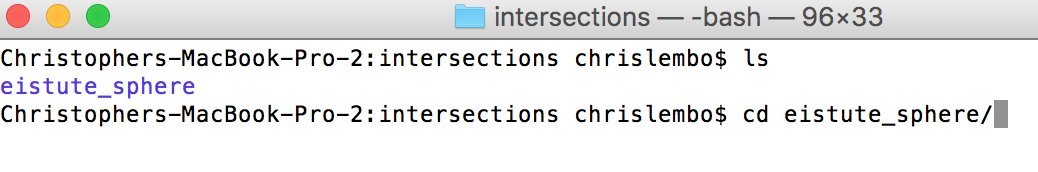
\includegraphics[width=0.4\textwidth]{curvesampler1}  \\  \\  \\
\hline \\
Invoke {\tt bertini} and {\tt bertini\_real} by entering in each on the command line individually & 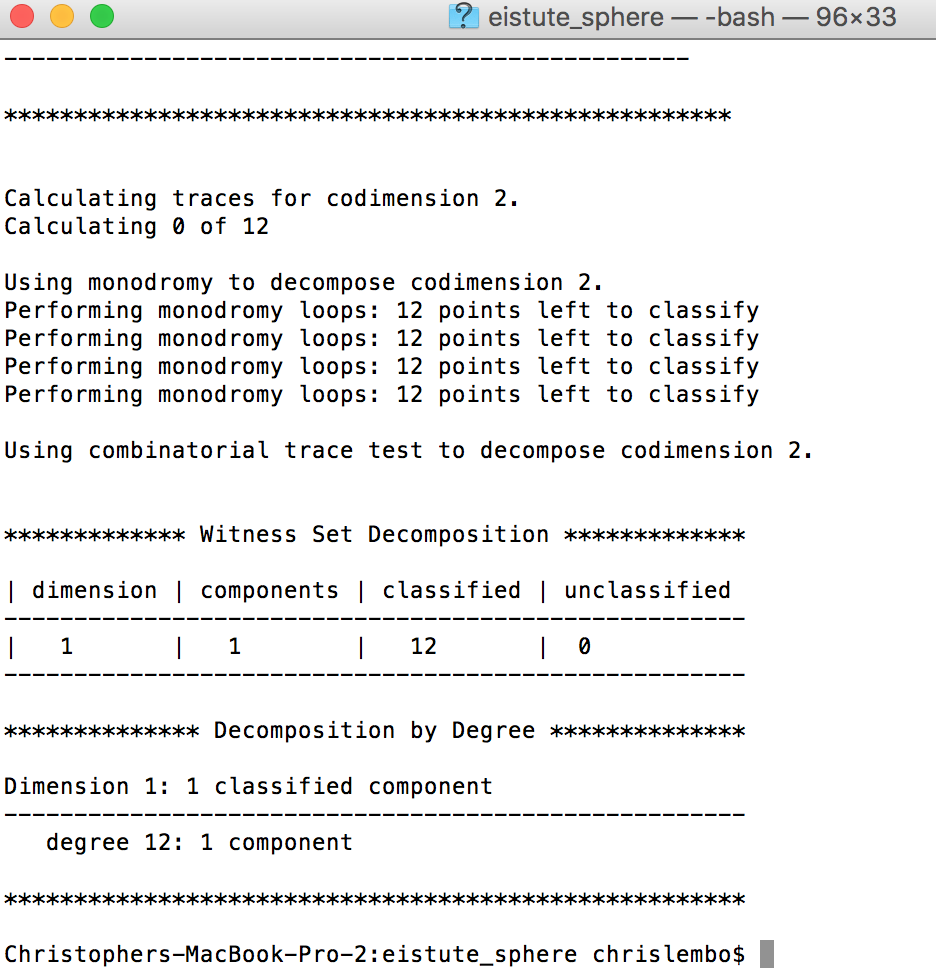
\includegraphics [width=0.4\textwidth]{curvesampler2} \\ \\ \\ 
\hline \\
Invoke {\tt sampler} by entering it in on the command line & 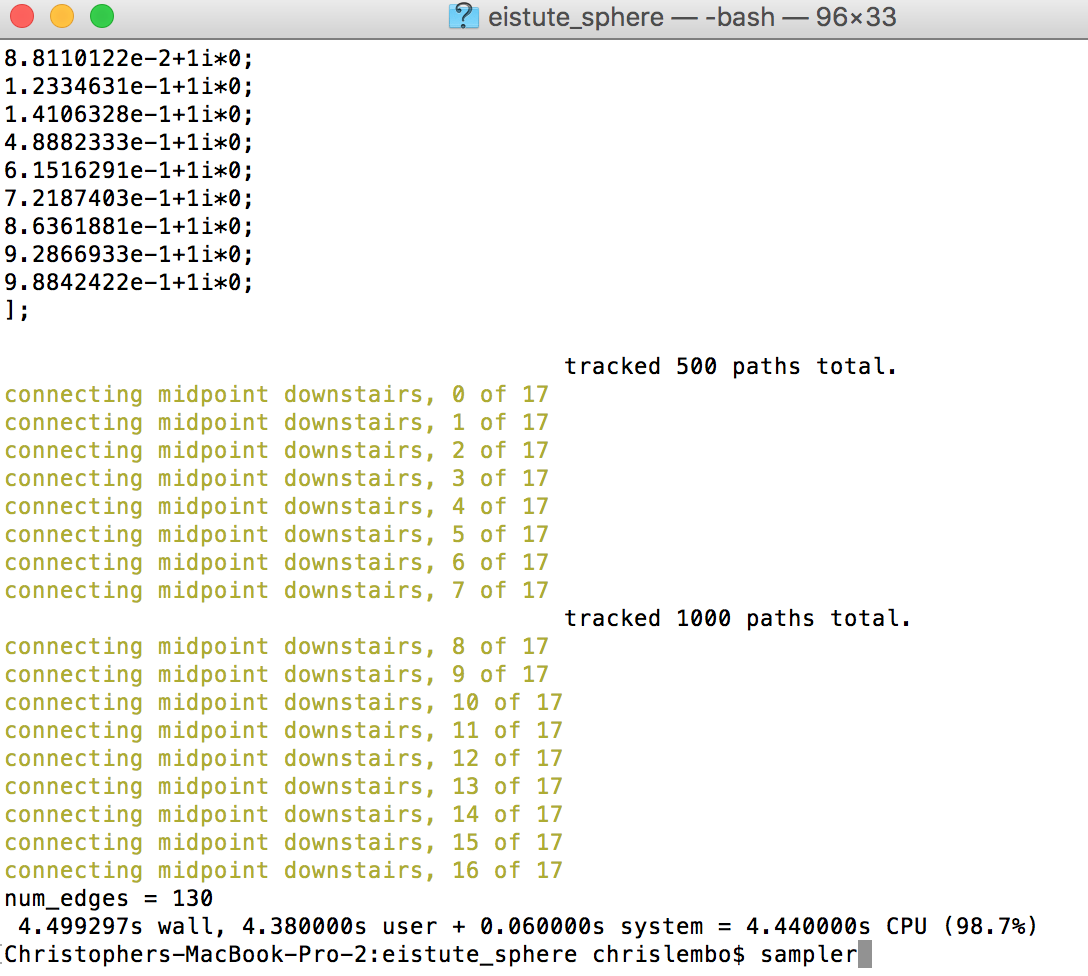
\includegraphics [width=0.4\textwidth]{curvesampler3} \\ \\ \\
\hline \\ 
Now use Matlab to produce the image of the curve
\begin{enumerate} 
	\item Go to the folder that holds your curve, then type {\tt gather\_br\_samples}
	\item To produce the image, type in {\tt bertini\_real\_plotter}
	\item you should end up with a figure along with matlab's display of viewing options
\end{enumerate}
& 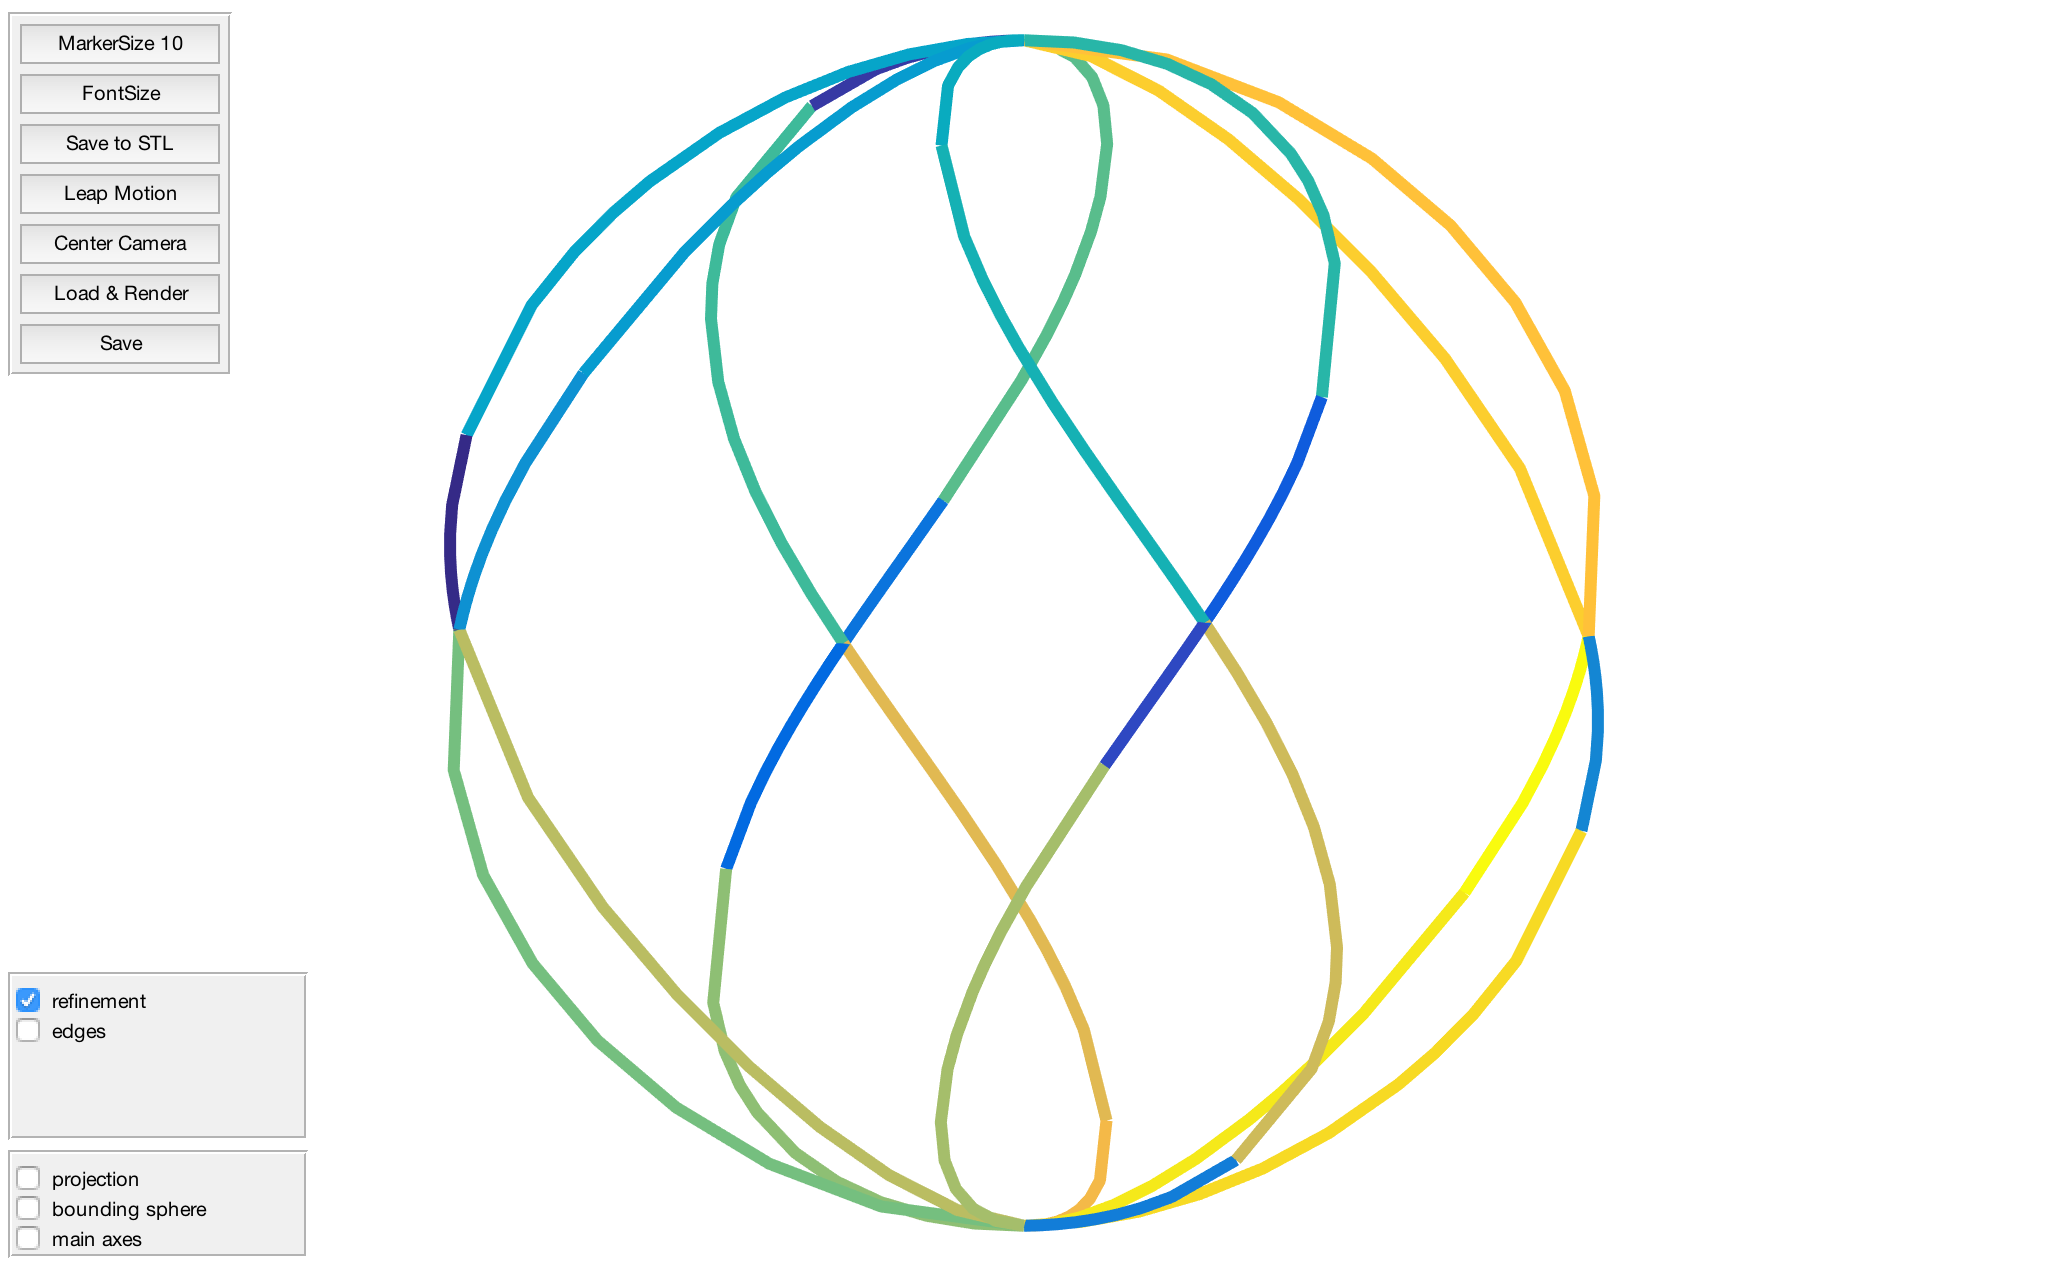
\includegraphics [width=0.4\textwidth]{curvesampler4.png} \\ \\ \\ 
  
\end{longtabu}


 	\subsubsection{Available curve sampling algorithms}
 	

 	There are three curve sampling algorithms available in the Sampler module for Bertini\_real.

 	\begin{enumerate}

 		\item {\tt -m [a]} -- Adaptive -- by movement of a predicted point.  Default choice.

 		\item {\tt -m d} -- Adaptive -- by distance between consective samples

 		\item {\tt -m f} -- Fixed -- every edge gets the same number of points

 	\end{enumerate}

The modes are accessed by calling sampler with the appropriate mode switch.


\paragraph{Curve sampling algorithm: Adaptive by movement}

This algorithm refines edge-by-edge until the predicted point, and the computed point, are close to each other.  It reduces sample density in regions of the curve which are flat, and has higher density in regions of high curvature.


\begin{figure}[H]
\begin{center}
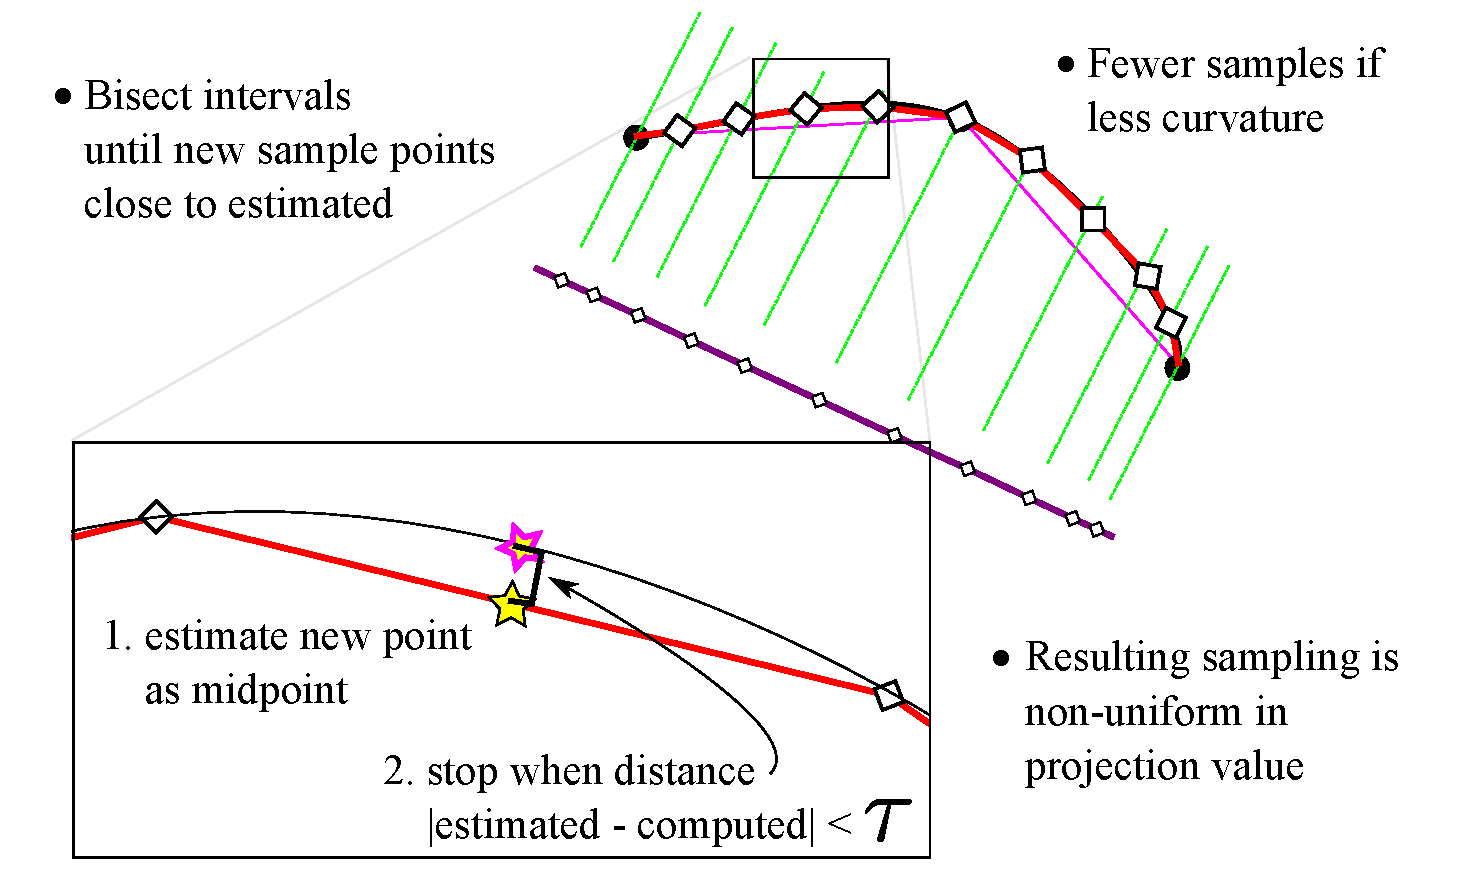
\includegraphics[scale = 0.4]{curve_sampling_adaptive_movement}
\caption[Adaptive-movement curve sampling]{Sampling a curve using movement-adaptive method.  New points are computed on the curve by bisecting intervals until the distance between the estimated midpoint and actual midpoint is less than convergence threshold $\tau$.}
\end{center}
\end{figure}
 

\begin{figure}[!htb]\centering
     \frame{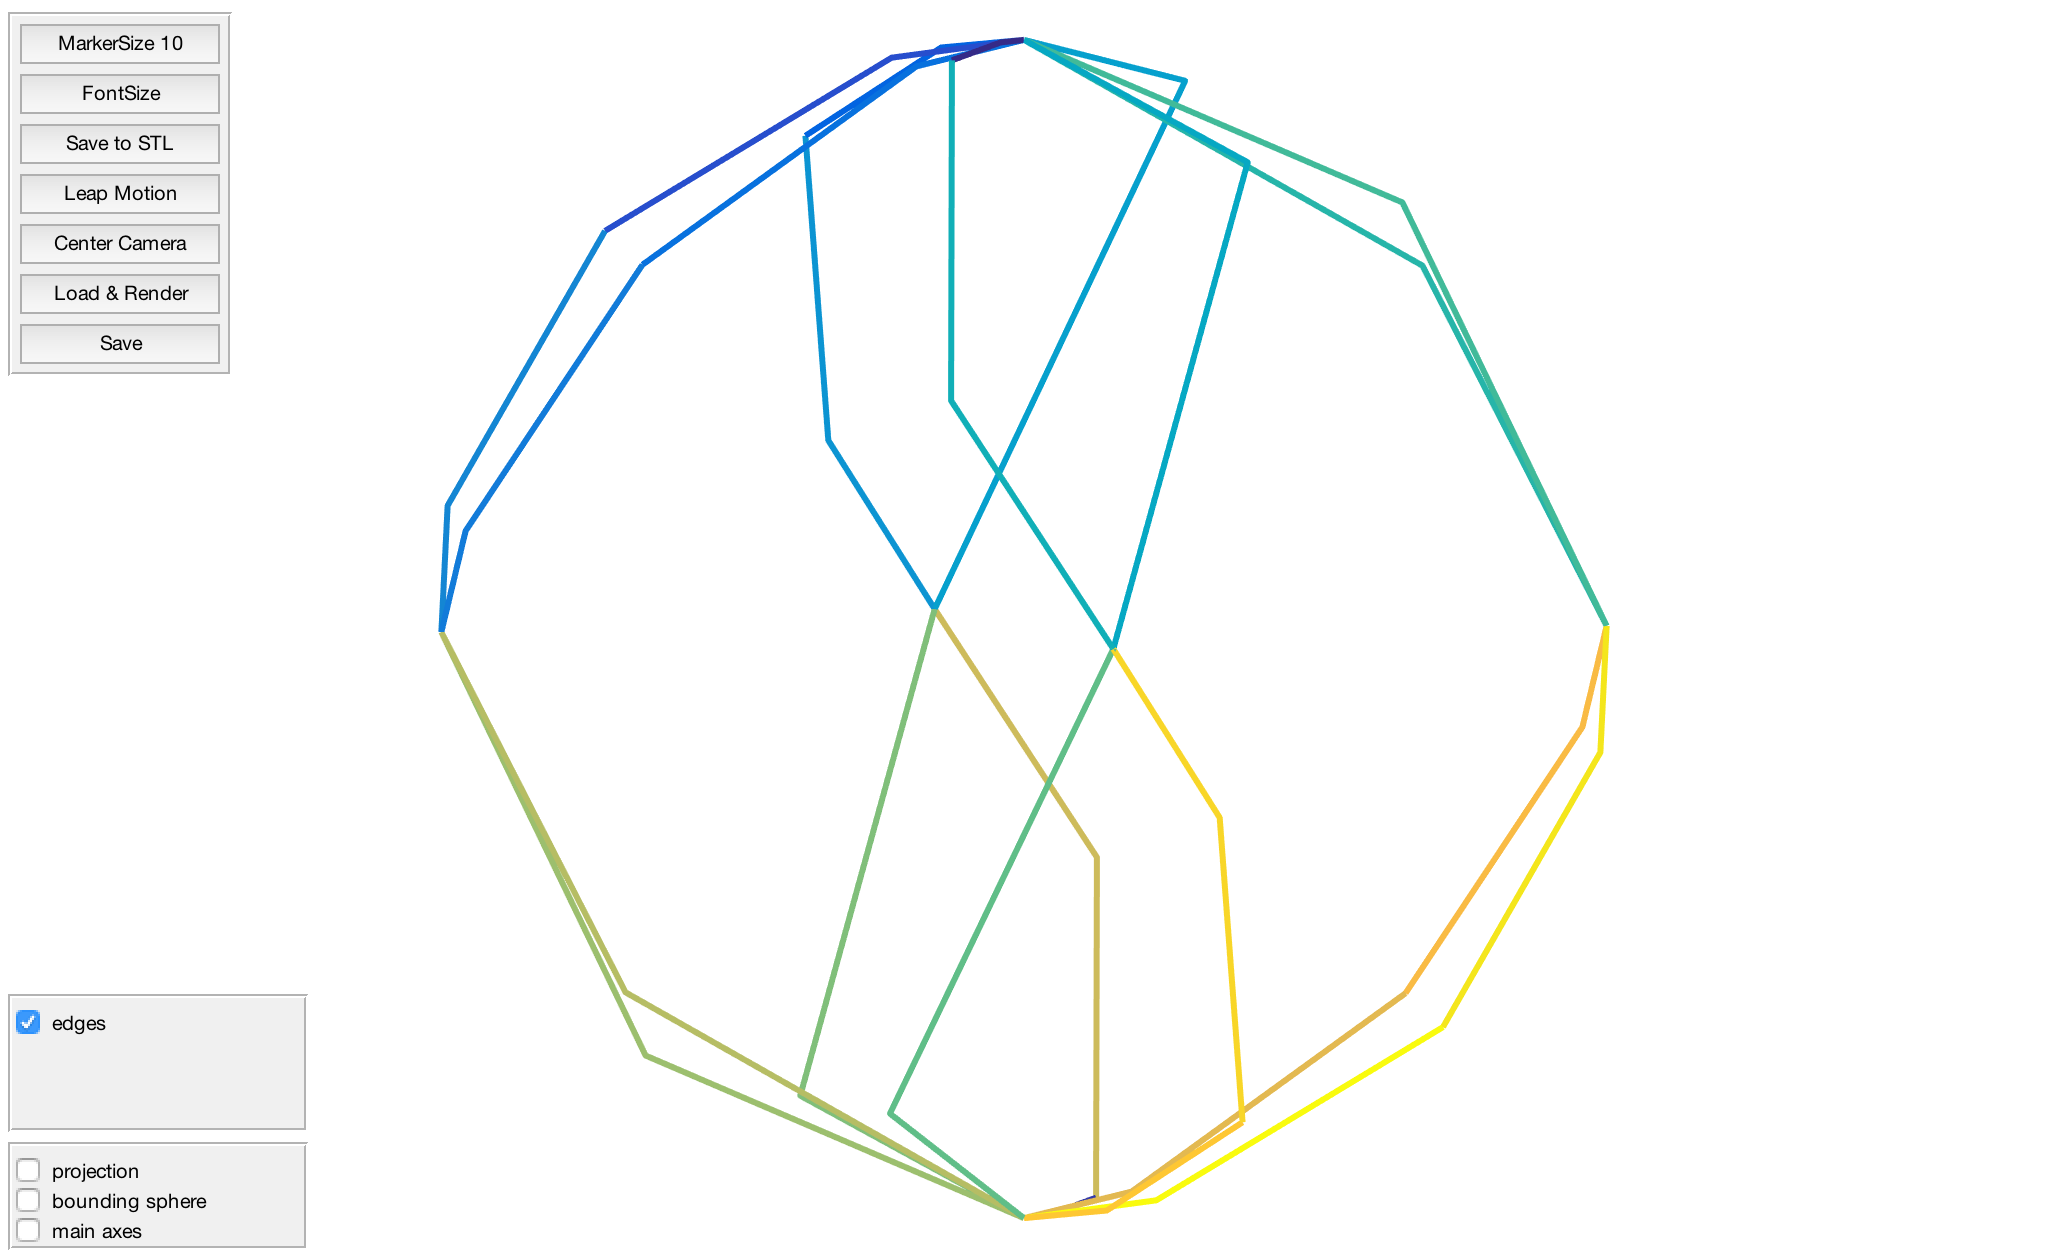
\includegraphics[width=10cm]{curvesampler_adm.png}}
     \caption{This is an example of sampling a curve using the adaptive by movement mode. To replicate this, when invoking sampler, type in {\tt sampler -m a}}
\end{figure}


\paragraph{Curve sampling algorithm: Adaptive by distance}

The adaptive-by-distance refinement algorithm refines the edge by bisection until the distance between consecutive samples is less than some user-set threshold, or a maximum number of refinement iterations has been computed.  This algorithm works well, but over-samples flat regions of the curve, where relatively few points should be necessary.  


\begin{figure}[H]
\begin{center}
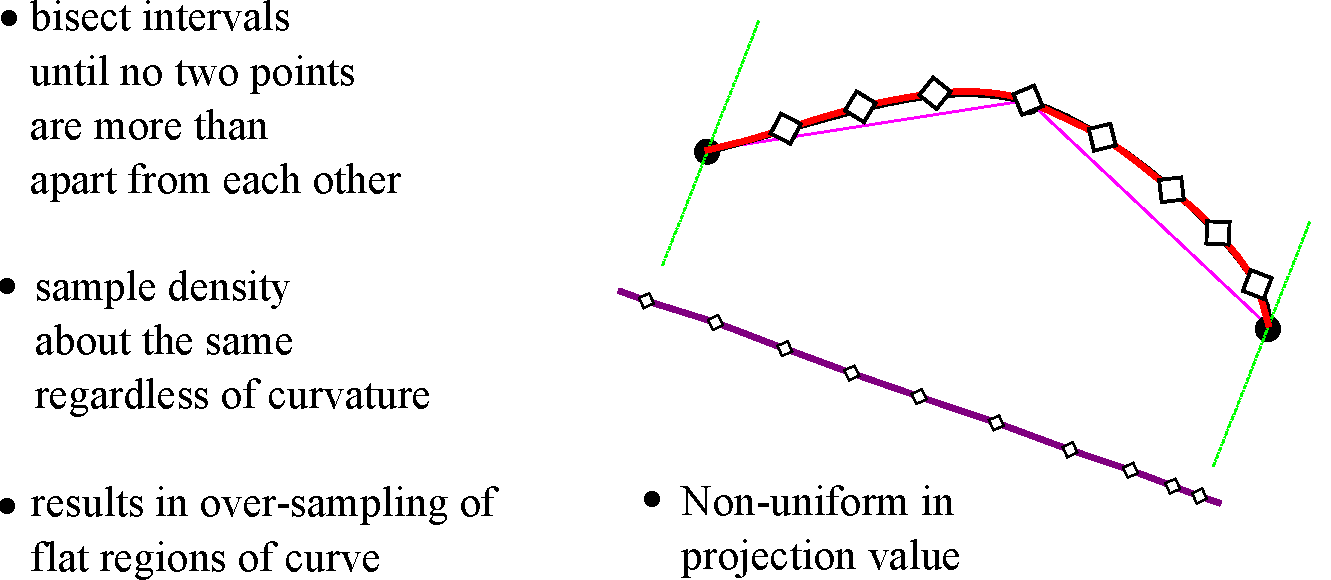
\includegraphics[scale = 0.4]{curve_sampling_adaptive_distance}
\caption[Adaptive-distance curve sampling]{Sampling a curve using distance-adaptive method.  New points are computed on the curve by bisecting intervals for which the distance between consecutive samples is larger than the convergence threshold $\tau$.}
\end{center}
\end{figure}

\begin{figure}[!htb]\centering
     \frame{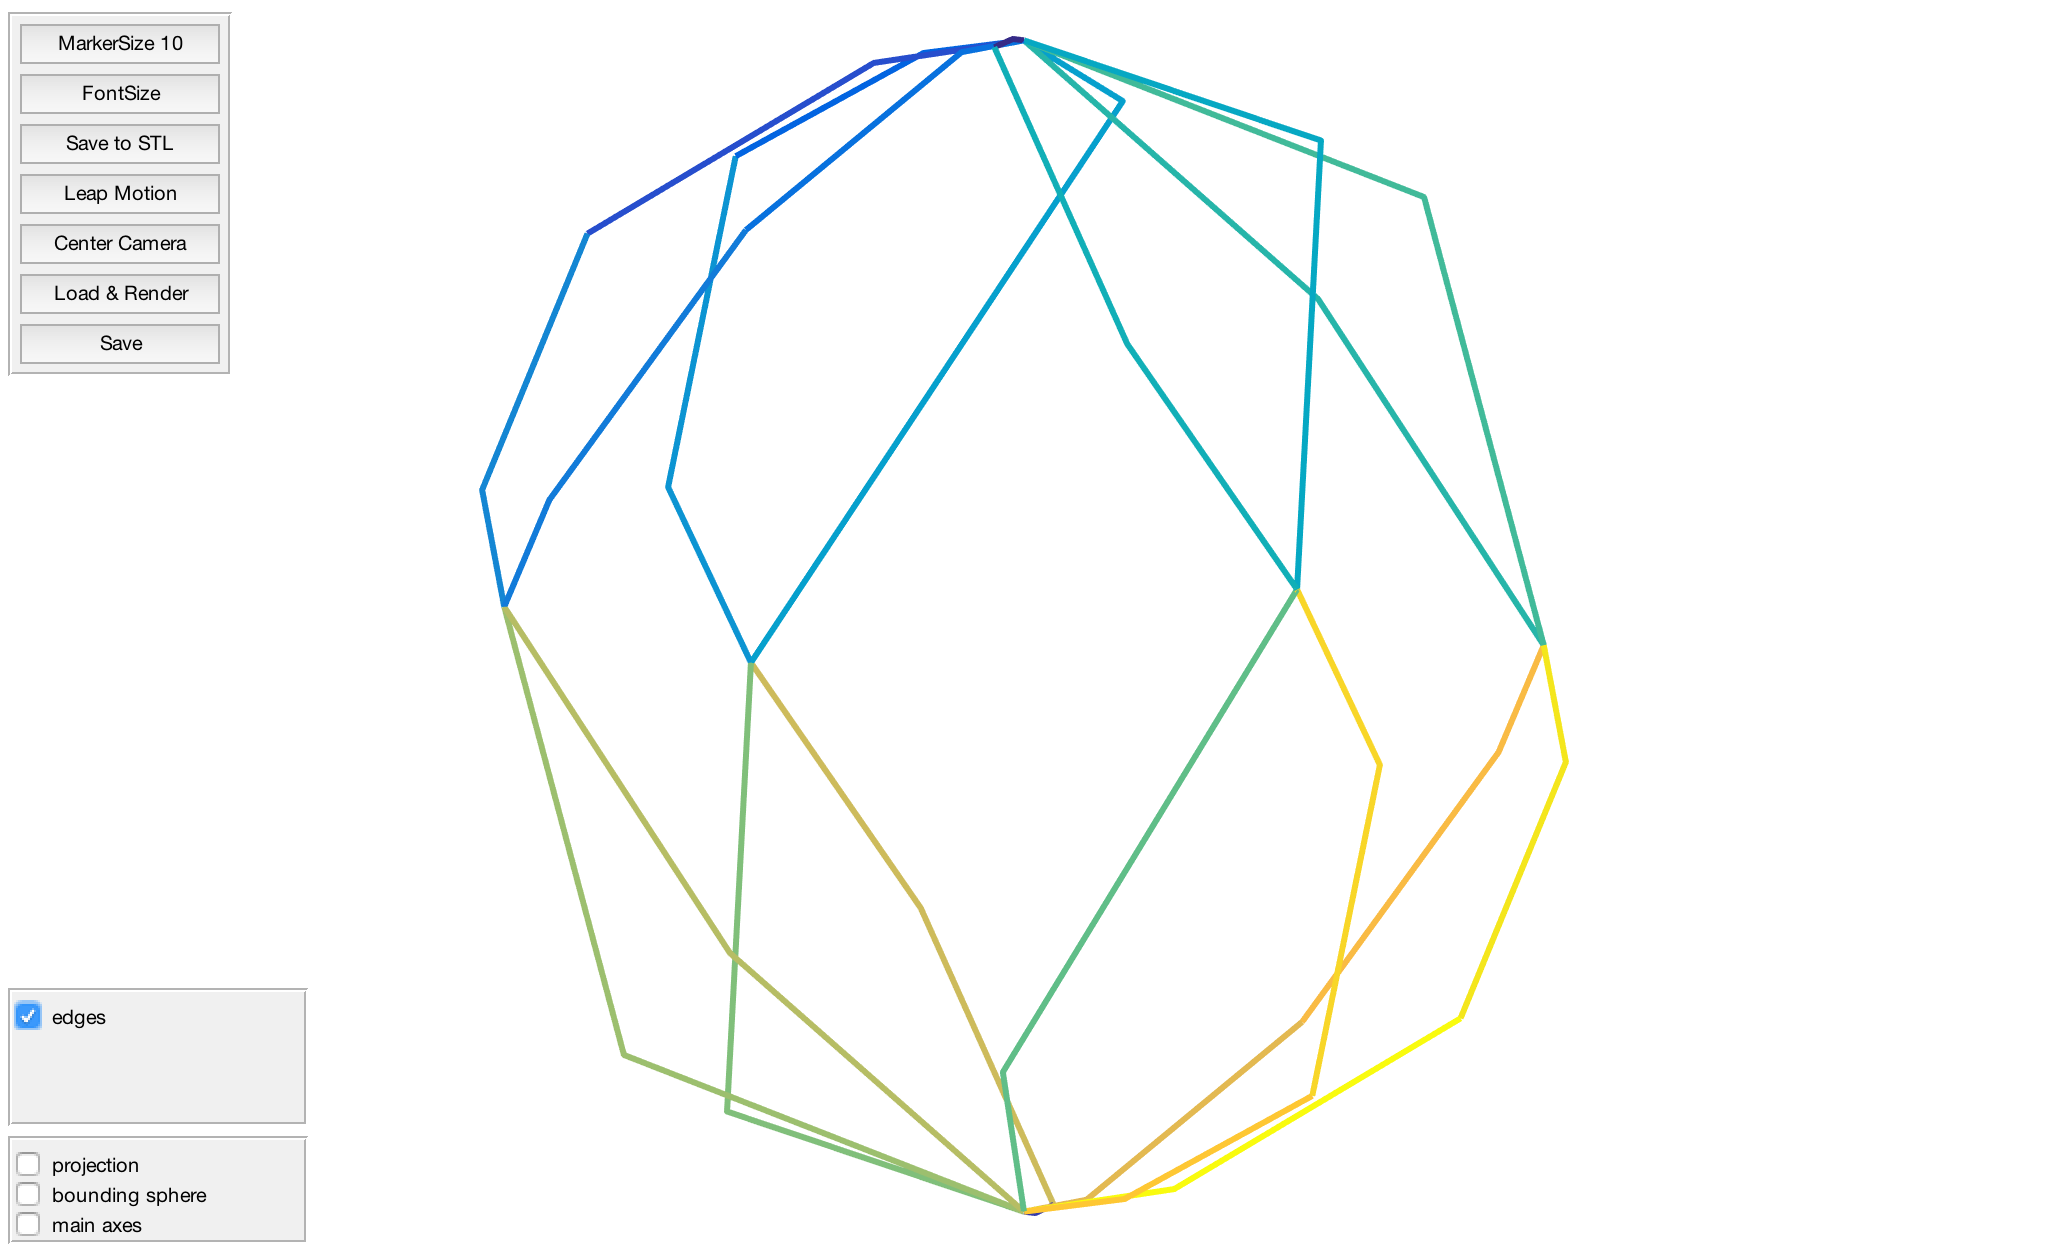
\includegraphics[width=10cm]{curvesampler_add.png}}
     \caption{This is an example of sampling a curve using the adaptive by distance mode. To replicate this, when invoking sampler, type in { \tt sampler -m d}}
\end{figure}

\paragraph{Curve sampling algorithm: Fixed number}

This curve sampling algorithm produces a fixed (by the user) number of sample points per edge of the decomposed curve.  


\begin{figure}[H]
\begin{center}
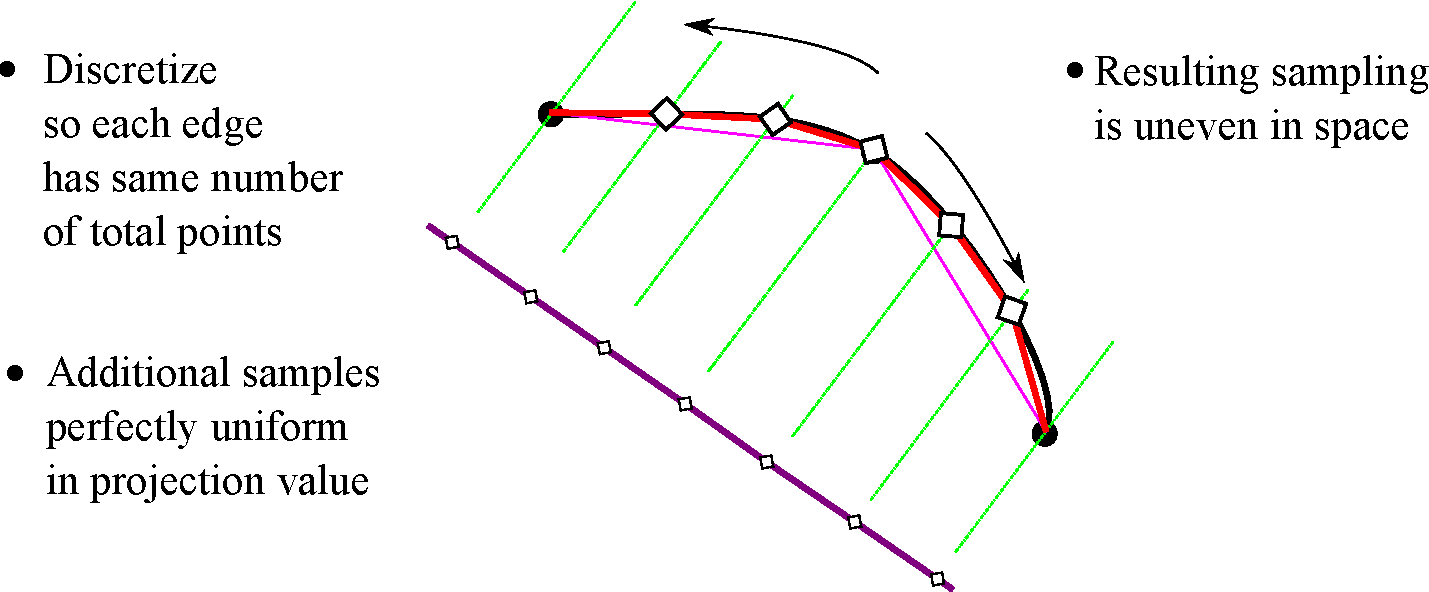
\includegraphics[scale = 0.4]{curve_sampling_fixed}
\caption[Fixed-number sampling of a curve -- how it works]{Fixed-number sampling of a curve.  The midpoint is homotoped so that a fixed number of sample points are computed on each edge of the curve.  The sample points are spaced uniformly in projection value, not in space.}
\end{center}
\end{figure}

\begin{figure}[!htb]\centering
     \frame{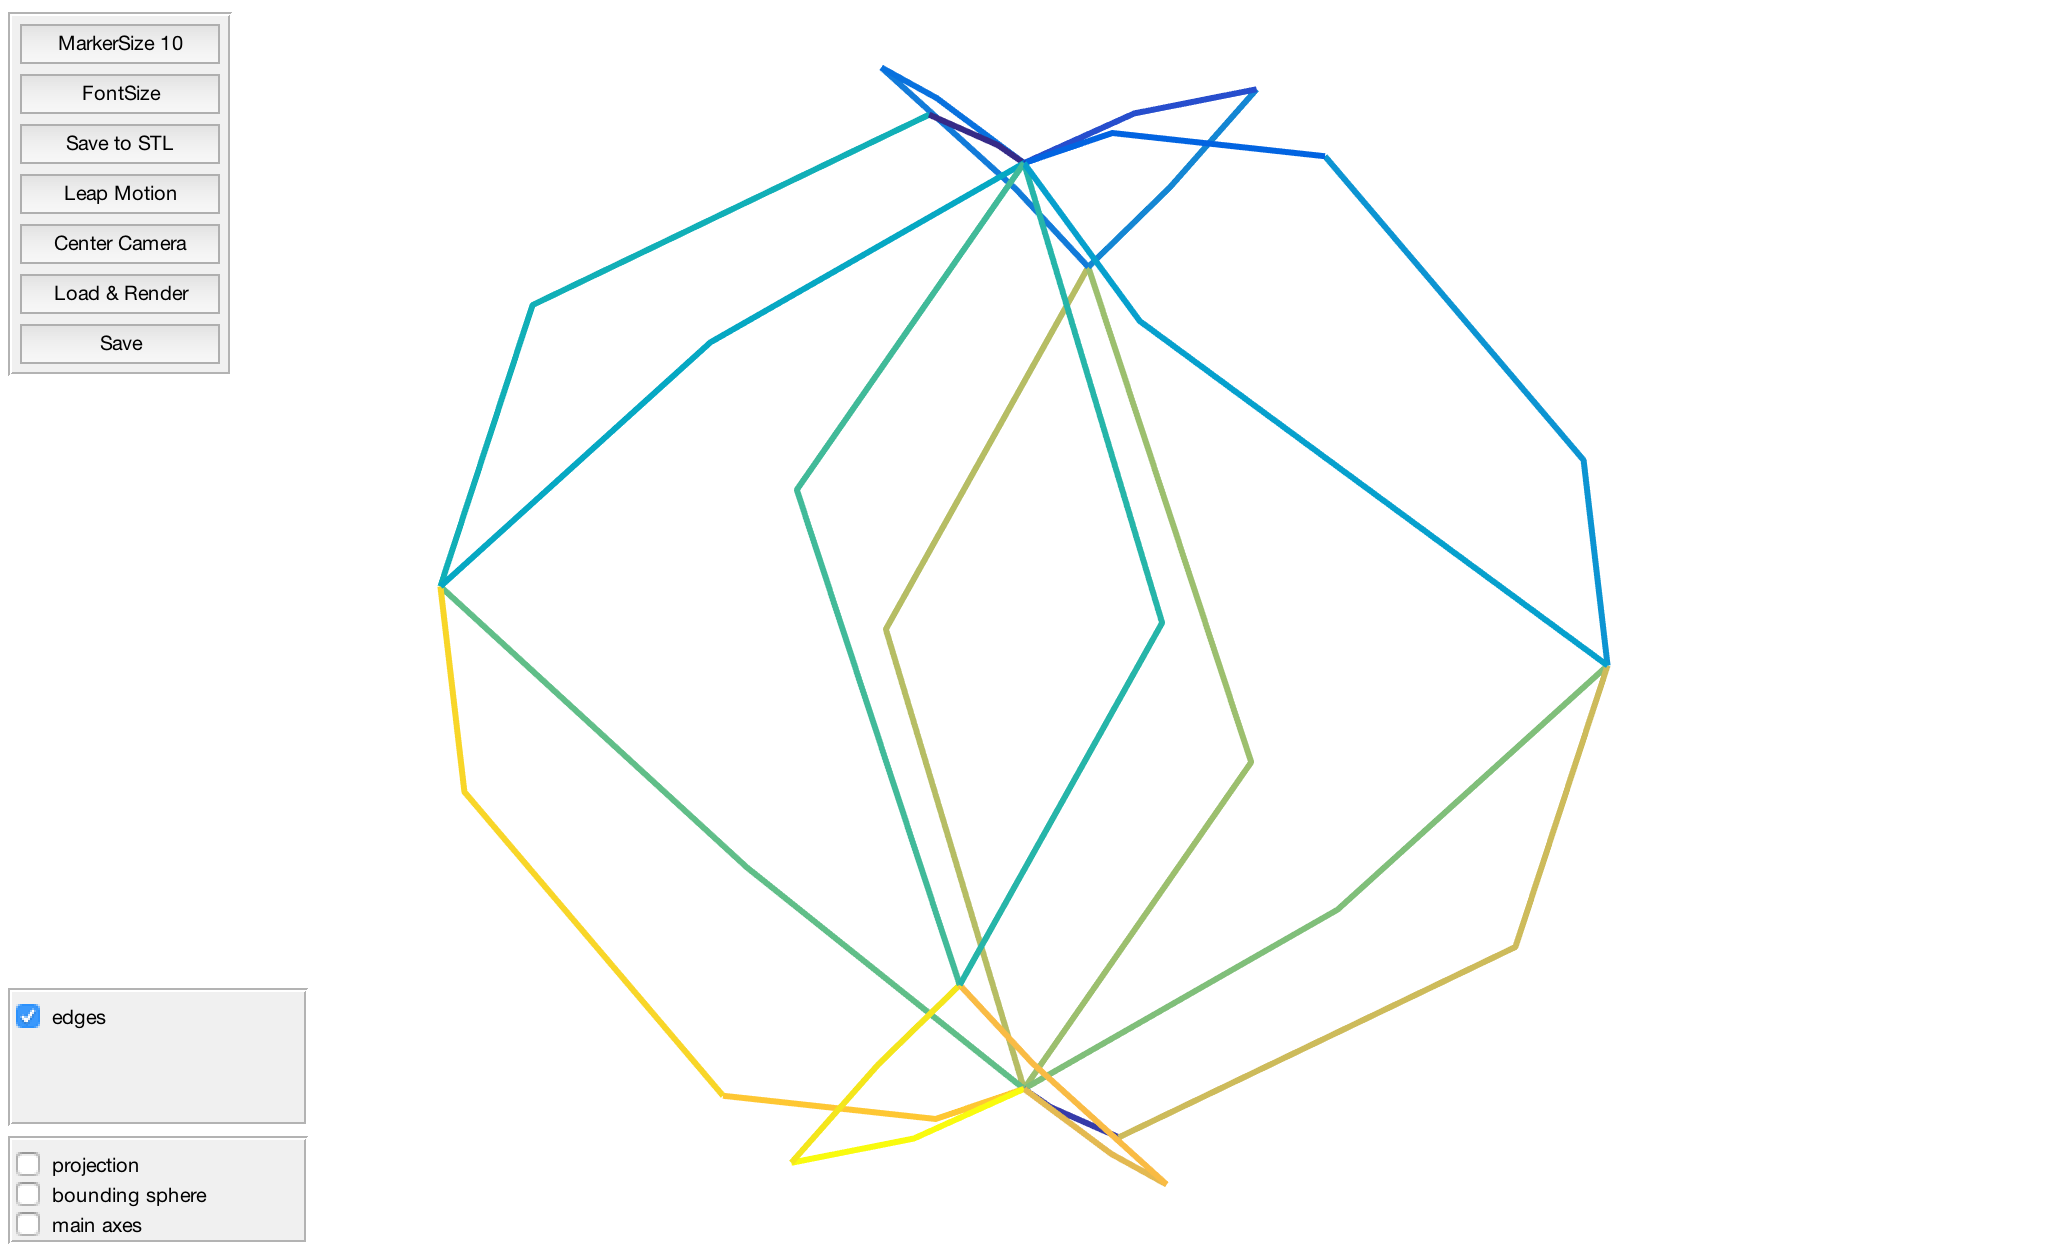
\includegraphics[width=10cm]{curvesampler_f.png}}
     \caption{This is an example of sampling a curve using fixed mode. To replicate this, when invoking sampler, type in {\tt sampler -m f}}
\end{figure}


\subsection{Surfaces}
\label{sec:sampler_surface}

\subsubsection{Running {\tt sampler} on a surface (Using an Example)}

This section will guide you through running sampler using a surface.\footnote{This content prepared by Chris Lembo.  Thanks Chris!}
 One thing to note is that it may take longer to invoke the sampler when using it on surfaces due to the amount of computation being done.

\begin{longtabu} to \textwidth {
 X[1,c,m]
 X[1,c,m]}
\hline
\rowfont\bfseries
\textbf{Instructions} & \textbf{Screen Shot} \\
\hline  \\ 
\endfirsthead
\caption[]{\textit{Continued from previous page}}\\
\hline
\textbf{Instructions} & \textbf{Screen Shot} \\
\hline \\
\endhead
\bottomrule \multicolumn{2}{r}{\textit{Continued on next page}} \\
\endfoot
\bottomrule \multicolumn{2}{r}{\textit{}} \\
\endlastfoot
First, choose the surface you wish to produce. (In this case I am choosing the {\tt sphere}, which is just found in the surfaces file. Once you enter into this file, you are ready to invoke:
\begin{itemize} 
\item {\tt bertini} 
\item {\tt bertini\_real} 
\item {\tt sampler}
\end{itemize} & 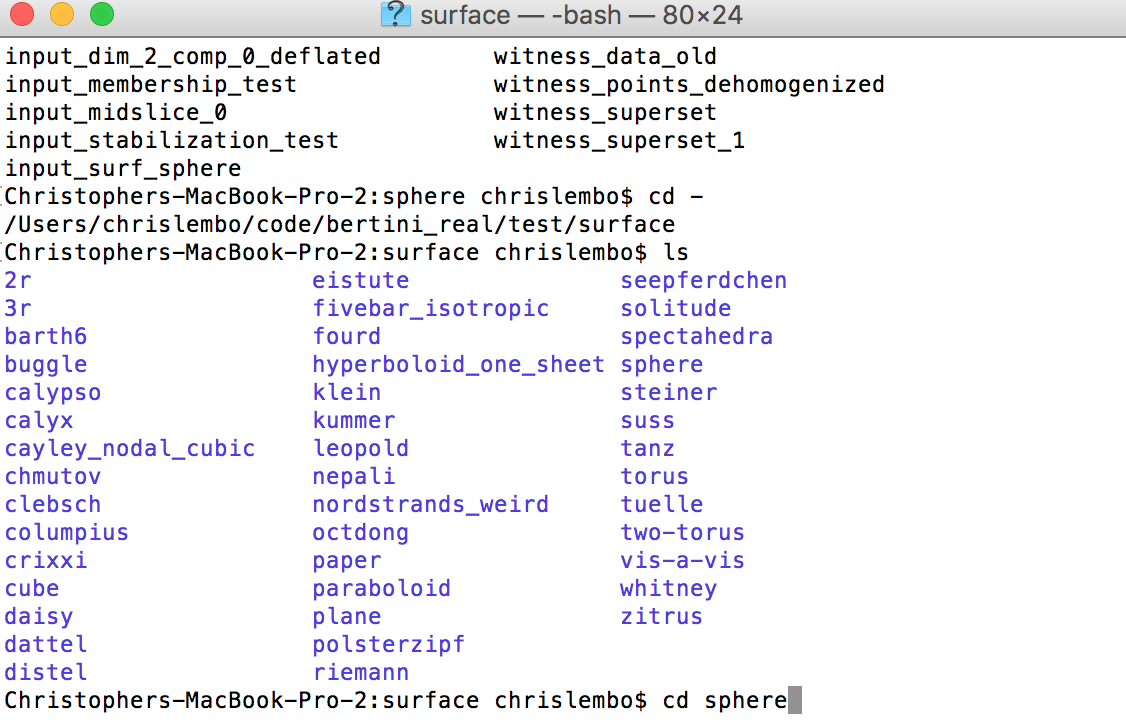
\includegraphics[width=0.4\textwidth]{surfacesampler1}  \\  \\  \\
\hline \\
Once sampler has been invoked, go to matlab and follow the same steps layed out for the sampler curve process, by gathering and plotting. Depending on refinements, you will end up with a sphere with fewer or more points. Here are the two matlab commands:
\begin{itemize} 
\item {\tt gather\_br\_samples} 
\item {\tt bertini\_real\_plotter}
\end{itemize}
 & 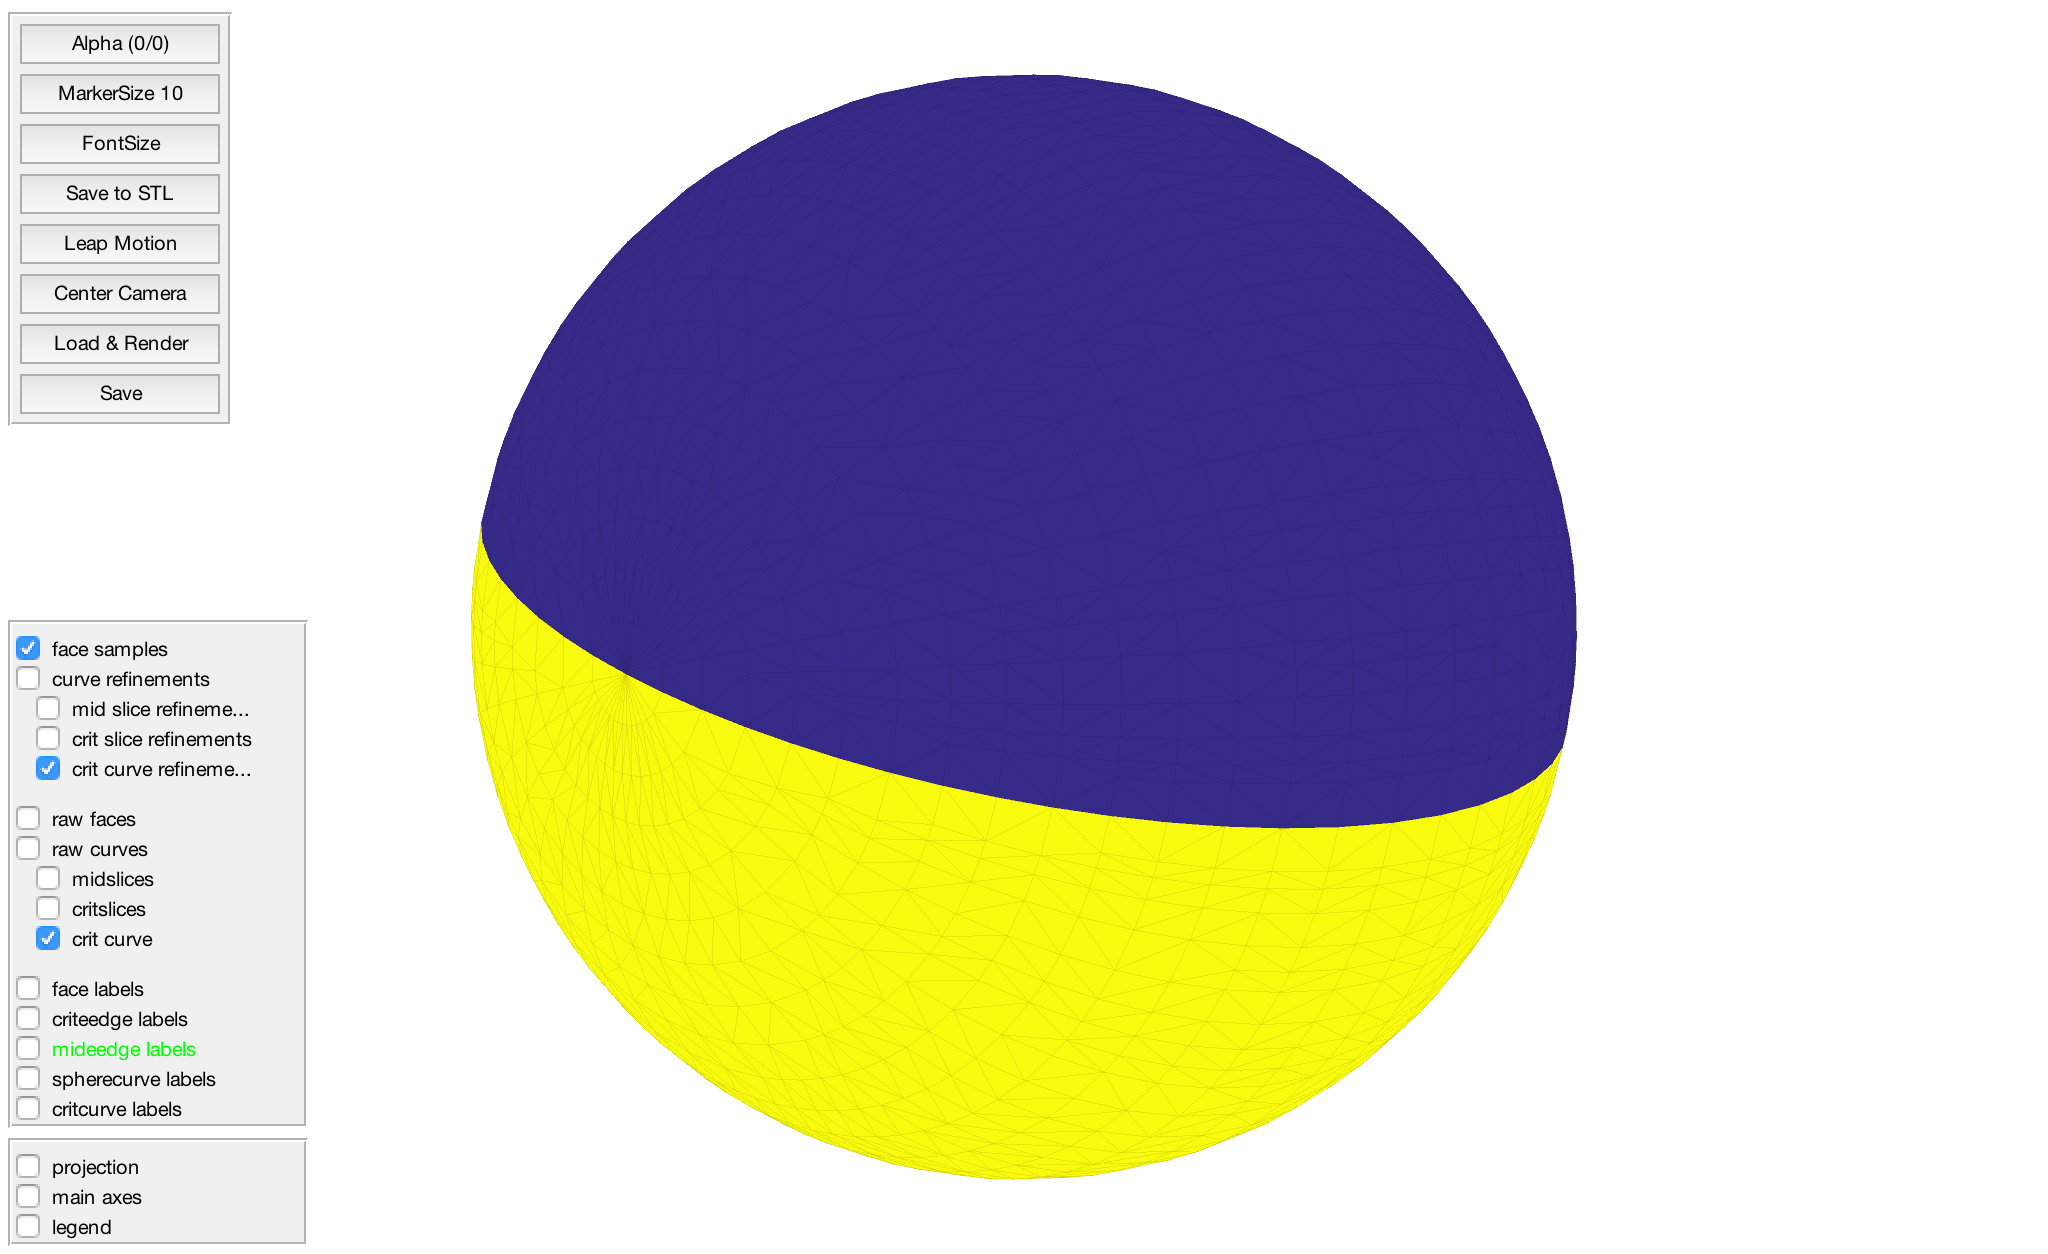
\includegraphics [width=0.4\textwidth]{surfacesampler2} \\ \\ \\   
\end{longtabu}






\subsubsection{Available surface sampling algorithms}


There are currently about two surface sampling algorithms, one of which is generally far superior to the other.  The inferior method is still maintained for posterity, because it produces interesting patterns on some surfaces, and is useful for instruction. 

\begin{enumerate}
\item {\tt -m [a]} – Adaptive-movement – Default choice.  Will be adaptive on distance moved, once it's implemented.  Sorry, we're not there yet on this one.
\item {\tt -m f} – Fixed – every edge of every critical-like curve gets the same number of points, and slices and ribs are sampled distance-adaptively.
\item {\tt -m [d]} – Adaptive-distance – Also default choice, because adaptive-movement collapses to the adaptive-distance method, until movement is implemented.  The sampling of critical-like curves are non-uniform, having somewhat-uniformly spaced samplings in terms of projection value across the entire curve.  Slices and ribs are distance-adaptively sampled.

\end{enumerate}

In short, the difference between distance-adaptive and fixed sampling is twofold:
\begin{itemize}

  \item Fixed sampling has the same number of `ribs' on each face, regardless of size.

  \item Fixed sampler currently linearly spaces sampled ribs.  Adaptive sampling spaces the ribs by cycle number, better approximating regions of the surface coming together at a singularity or critical point.  

\end{itemize}


\paragraph*{Commonalities}

\begin{figure}[H]
\begin{center}
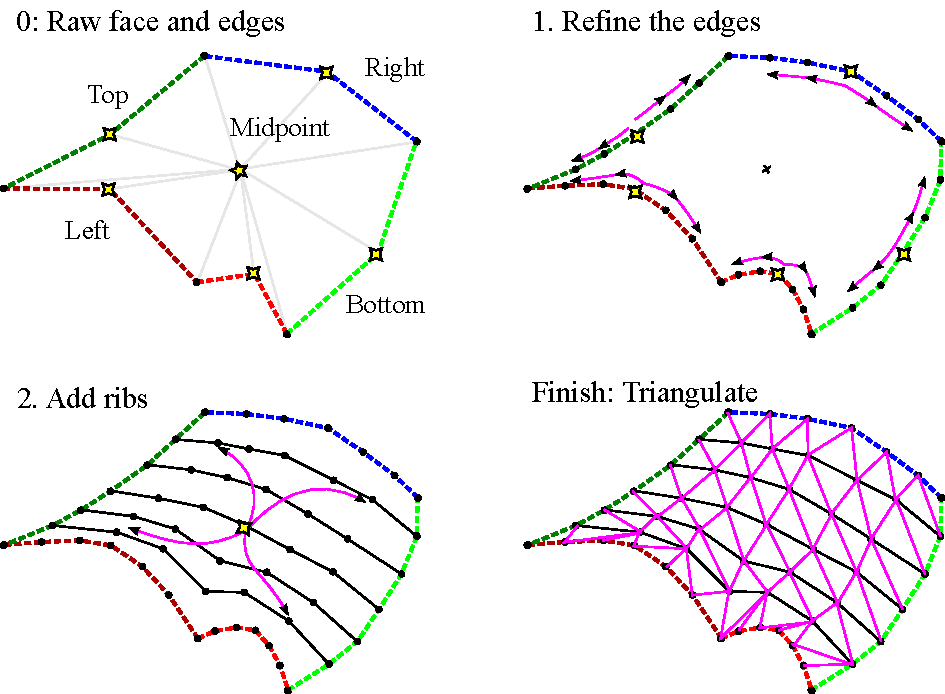
\includegraphics[width=4in]{surface_refinement}
\caption[Surface refinement]{Refining a surface, using the built-in refinement algorithms.  Edges of bounding curves are sampled, then the face is ribbed, then the triangulation stitched together.  A more familiar adaptive triangulation method from, e.g. computer vision, is not used because this can happen in higher ambient dimensions.}
\end{center}
\end{figure}

The current surface sampling algorithms are two-step methods:
\begin{enumerate}
\item Sample the curves using some combination of methods
\item Sample the faces themselves using some method
\end{enumerate}



Current methods also use what Dani calls `ribs'.  These are curves of samples across the interior of a face, all lying in the same fiber of $\pi_0$, so named because they look like ribs on an animal.  There are certainly better ways to sample a face.  However, the literature almost entirely describes 3D triangulations, and how to optimally form them.  Bertini\_real can compute triangulations in more coordinates, where many of the necessary ingredients are missing.  Research is necessary.  Collaborate!

In all surface sampling algorithms, new points in the surface are computed by exploiting the homotopy \eqref{eqn:midtrack} from Section~\ref{sec:connect_surface}.  We will first discuss the weaker of the two methods, because it is briefer and easier to explain.












\paragraph{Surface sampling algorithm: Fixed}

This surface sampler uses the following parameters:
\begin{itemize}[noitemsep]
\item {\tt numsamples}
\item {\tt tol}
\item {\tt minits}
  \item {\tt maxits}
\end{itemize}

In the fixed-number surface sampling algorithm, 
\begin{enumerate}
\item Each edge of each crit-like curve is sampled so it has the same number of points, {\tt numsamples}.  The samples are spaced evenly {\em in terms of projection value}, not space, linearly.  

\item Each mid- and critslice is refined using distance-adaptive curve sampler, until {\tt tol} distance is reached, or {\tt min/maxits} refinement iterations are used.

\item The faces are sampled using the distance-adaptive curve method, again using {\tt tol} and {\tt min/maxits}
\end{enumerate}

This method produces mediocre samplings around singularities, because there is too much space between ribs near the challenge points.  The adaptive methods are much better at producing a ``smooth'' sampling, because they use the cycle number of the critical points.


\begin{figure}[!htb]\centering
     \frame{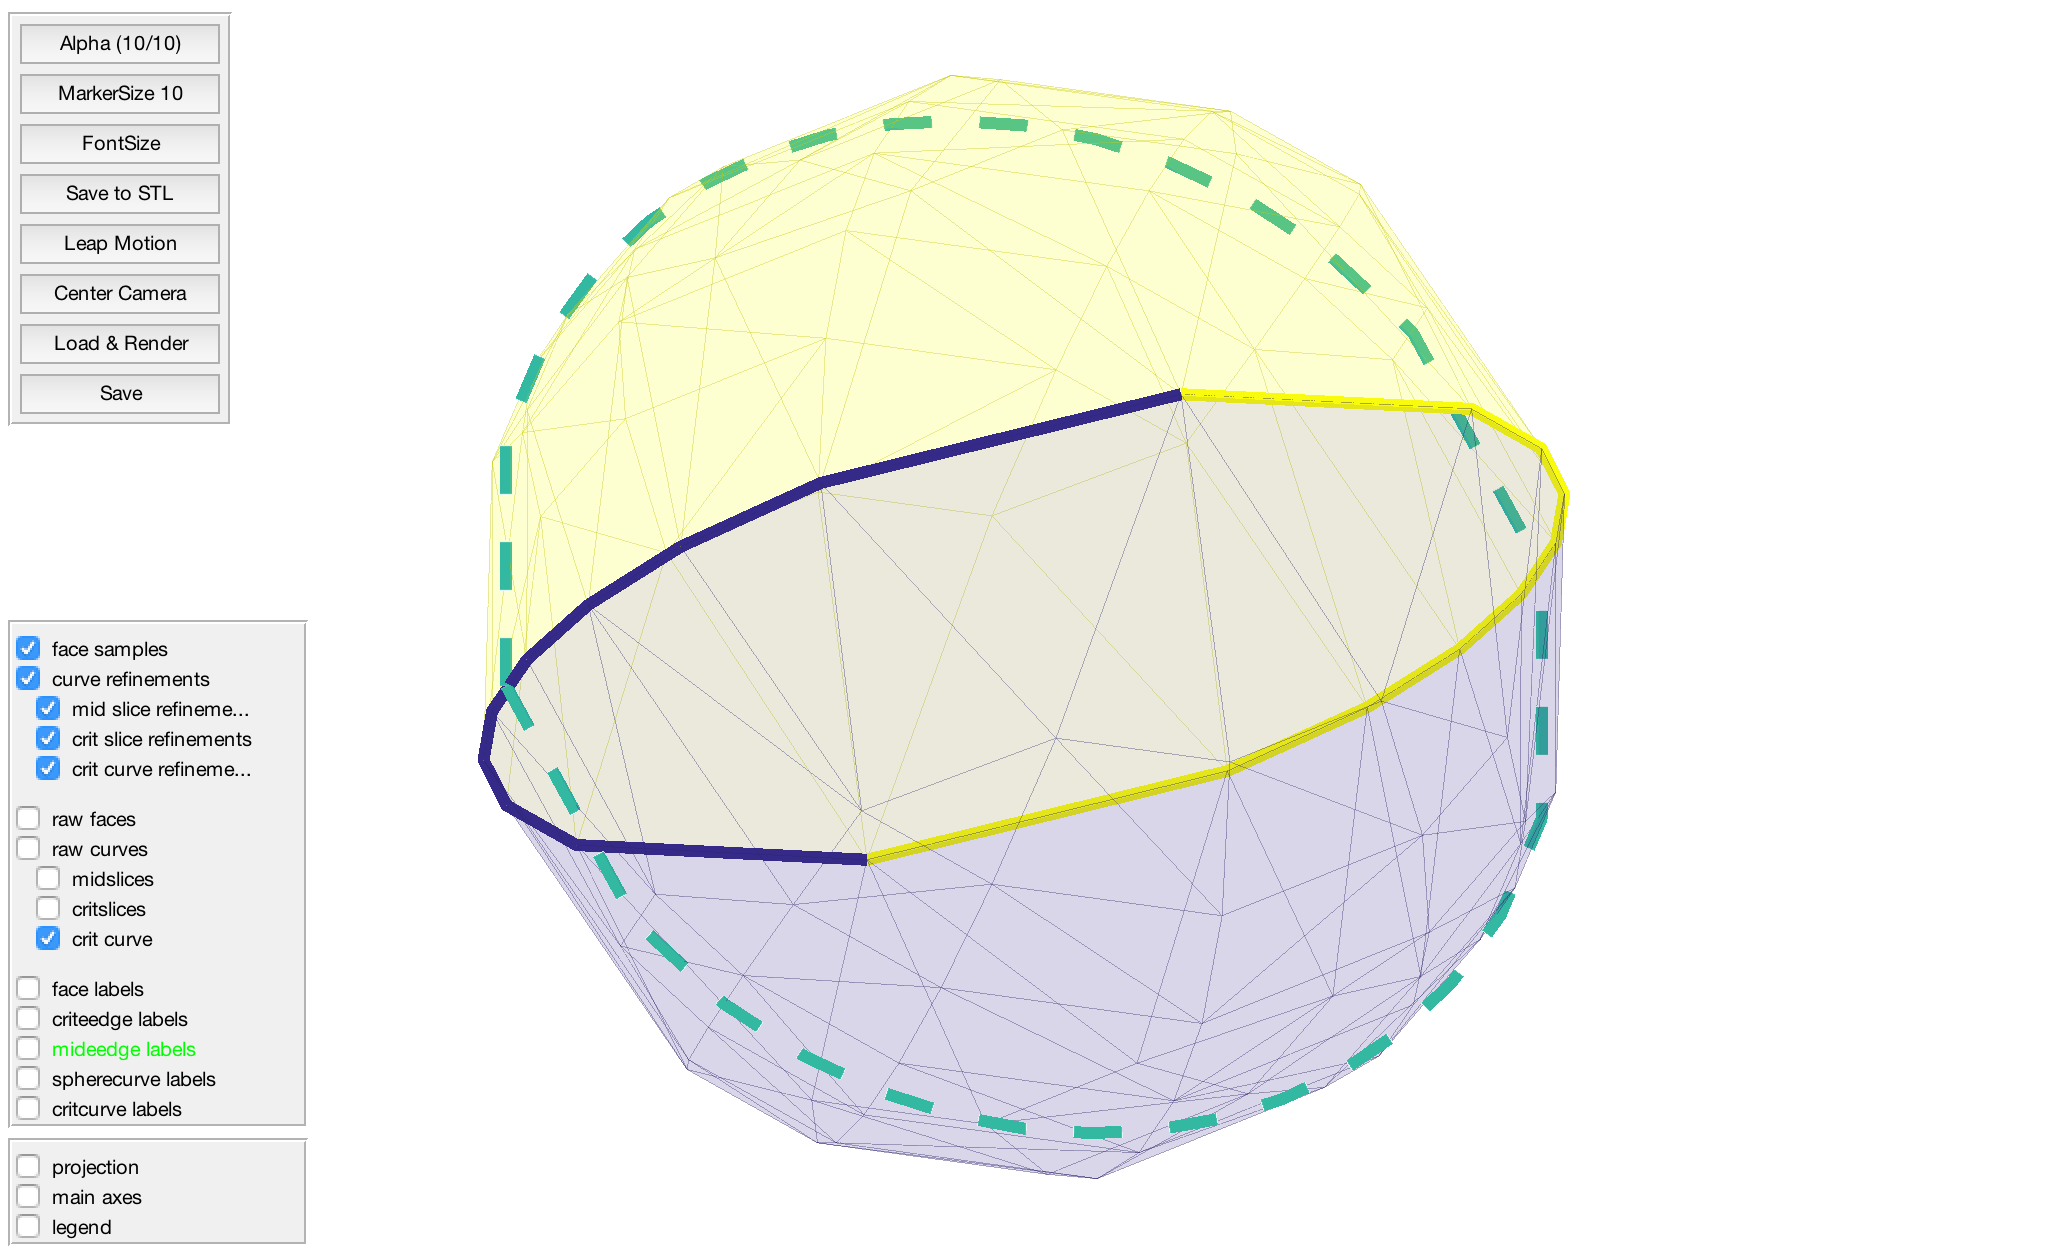
\includegraphics[width=10cm]{surfacefixed_numsamples.png}}
     \caption{This is an example of sampling a surface using the fixed numsamples mode. To replicate this, when invoking sampler, type in {\tt sampler -m f numsamples 5 -tol 0.7}}
\end{figure}

\begin{figure}[!htb]\centering
     \frame{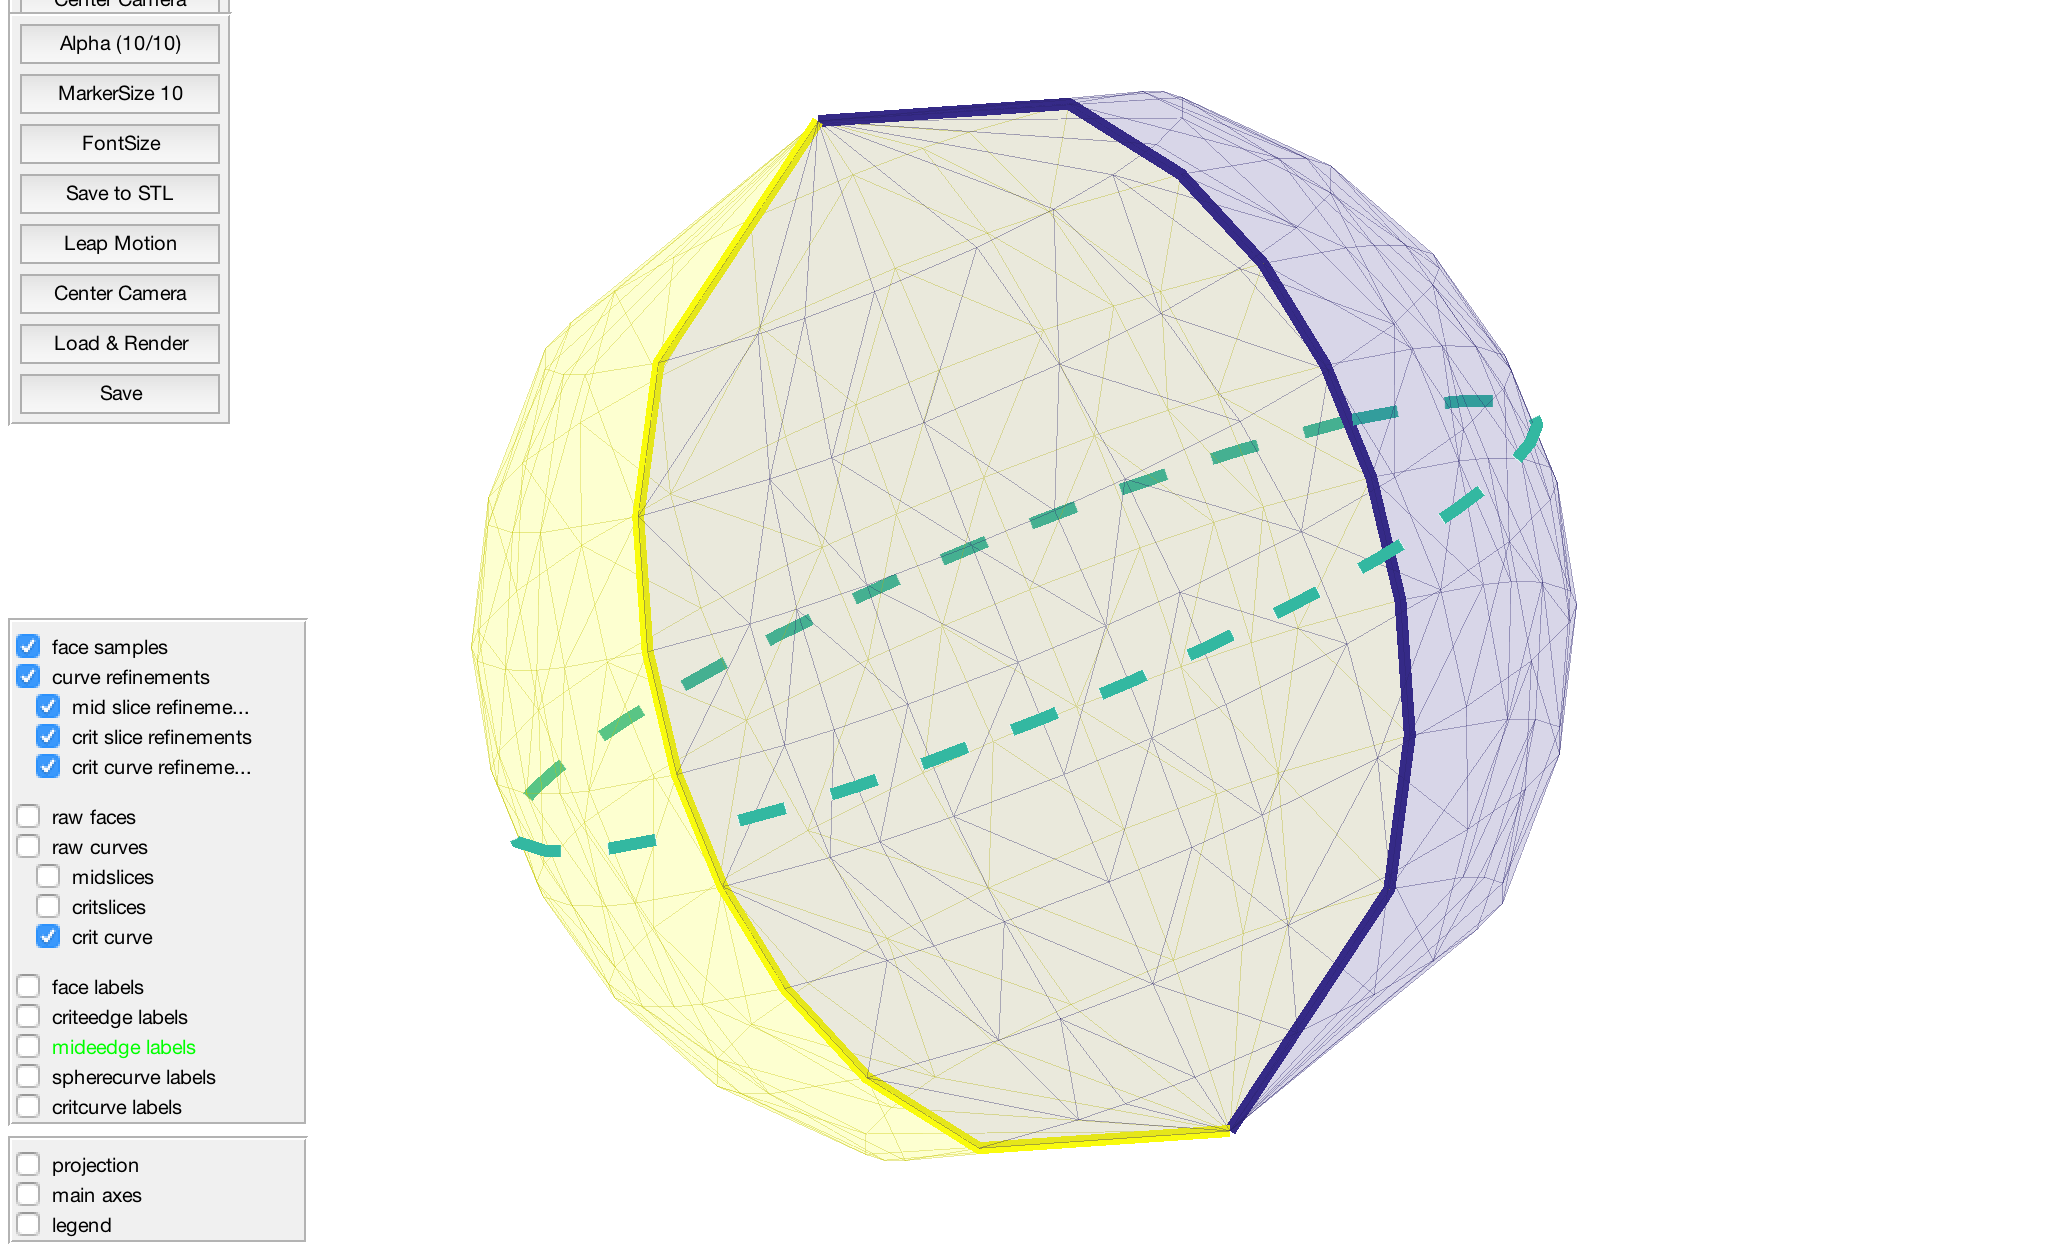
\includegraphics[width=10cm]{surfacefixed_minits.png}}
     \caption{This is an example of sampling a surface using the fixed minits mode. To replicate this, when invoking sampler, type in {\tt sampler -m f minits 5 -tol 0.3}}
\end{figure}

\begin{figure}[!htb]\centering
     \frame{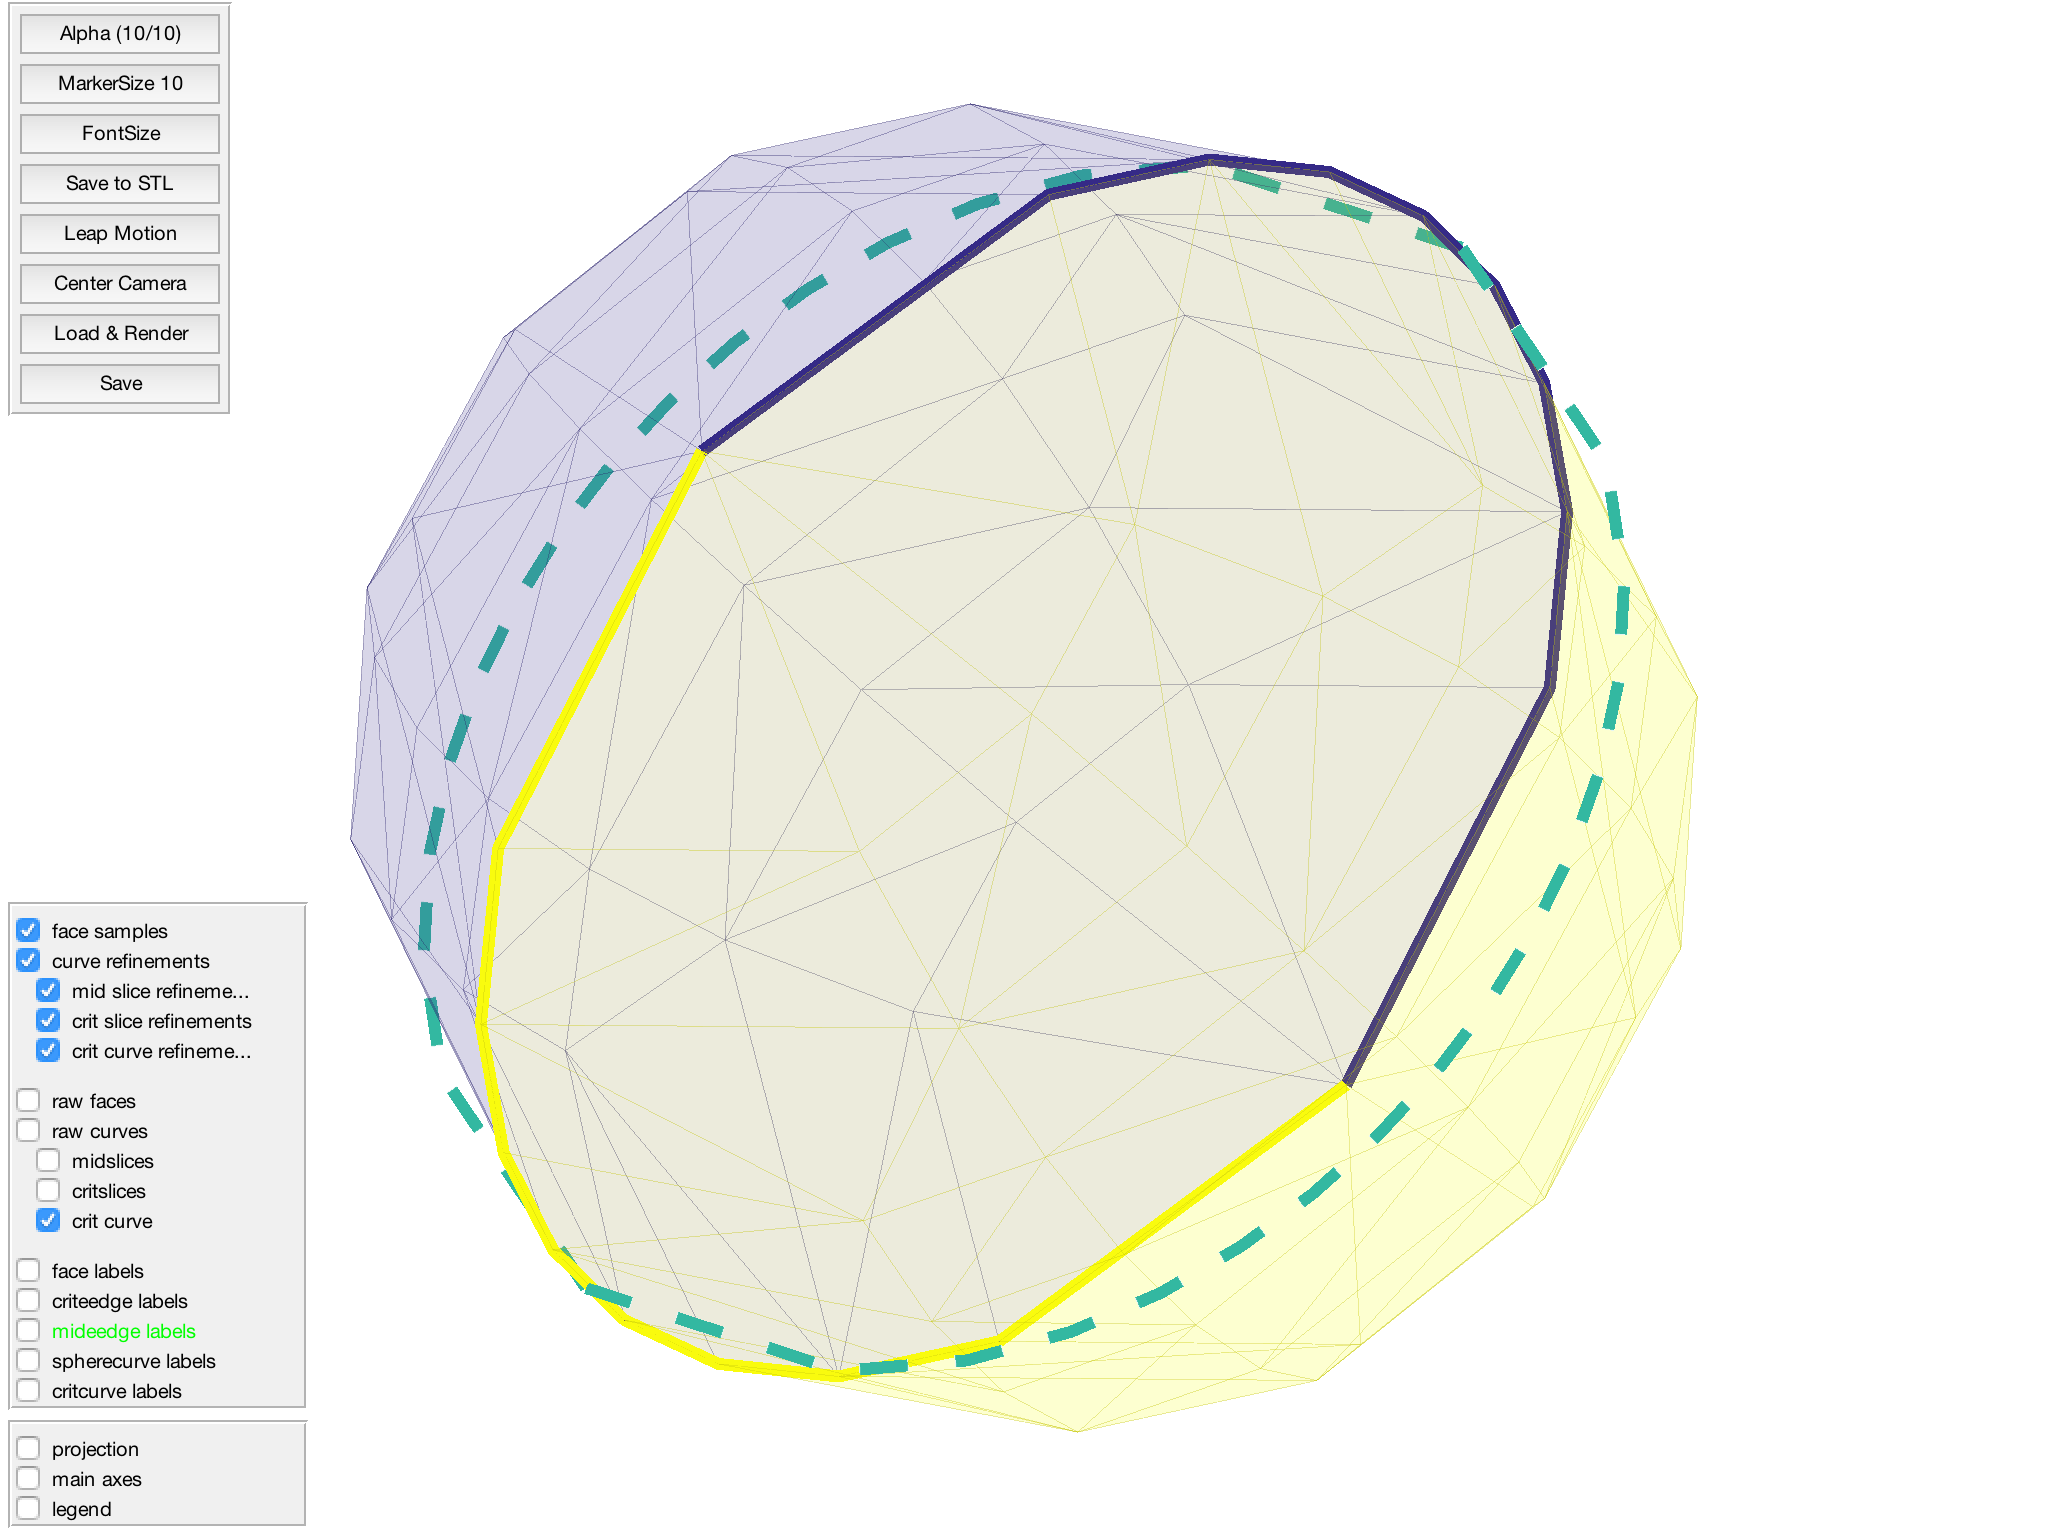
\includegraphics[width=10cm]{surfacefixed_maxits.png}}
     \caption{This is an example of sampling a surface using the fixed maxits mode. To replicate this, when invoking sampler, type in {\tt sampler -m f maxits 5 -tol 0.9}}
\end{figure}

\paragraph{Surface sampling algorithm: Adaptive by distance}

This surface sampler uses the following parameters:
\begin{itemize}[noitemsep]
  \item {\tt minribs}
  \item {\tt maxribs}
  \item {\tt minits}
  \item {\tt maxits}
  \item {\tt tol}
\end{itemize}


In the distance-adaptive surface sampler:
\begin{enumerate}
\item The crit-like curves are refined using a modified fixed-number sampler.  The number of samples per edge is uniform within a particular $\pi_0$ crit-interval, but different intervals will have different numbers of samples in them.  The number of samples $m$ in an interval is computed as
\begin{align*}
m_1 &= \text{max estimated length of crit edge} / \text{tol} \\
m_2 &= \min(m_1, \text{maxribs}) \\
m &= \max(m_2, \text{minribs})
\end{align*}
This means that wider edges will have more samples, narrower will have few.

We allow the capping of a max number of samples, because small {\tt tol} will lead to insanely large samplings of a complete surface.  We also allow a min number of samples, so that even small faces will get refined to some minimal level, which can be important around singularities.

The samples on the crit-like edges are non-linearly spaced, using the cycle number of the edge to space them.  That is, there is a special number, the cycle number $c$, which can be used to regularize a path.  This number is computed as a matter of course while curve decomposing, and hence we store it for use in the sampler routines.  Cycle number 2 means, approaching the boundary of an edge, each sample is square root as distant as the previous.  Cycle number 3 means it goes as the cube root.  Cycle number 1 produces linearly-spaced samples.  Ideally the cycle number used to space the samples, and hence ribs on faces, should me an integer multiple of all possible cycle numbers generated by all possible paths on the face, walking toward the boundary.

Presently, the cycle number is forced to be uniform across all edges of the entire surface, because allowing it to vary causes problems when adjoining adjacent faces with disparate cycle numbers.  If you want this feature, please consider collaborating with Dani to add it.

Also, the cycle number is presently hard-coded at 2.  Changing this to be a runtime-set parameter value should be pretty easy.  Let Dani know if this is a pressing issue for you.



\item  The mid- and critslices are refined using the distance-adaptive curve sampler.

\item The faces are ribbed at the $\pi_0$ projection values for the samples on the crit-like edges forming the top and bottom boundaries of the face.  The ribbing process is distance-adaptive, with a min and max number of allowable refinement iterations ({\tt minits}, {\tt maxits}) to achieve the desired tolerance {\tt tol}.
\end{enumerate}


\begin{figure}[!htb]\centering
     \frame{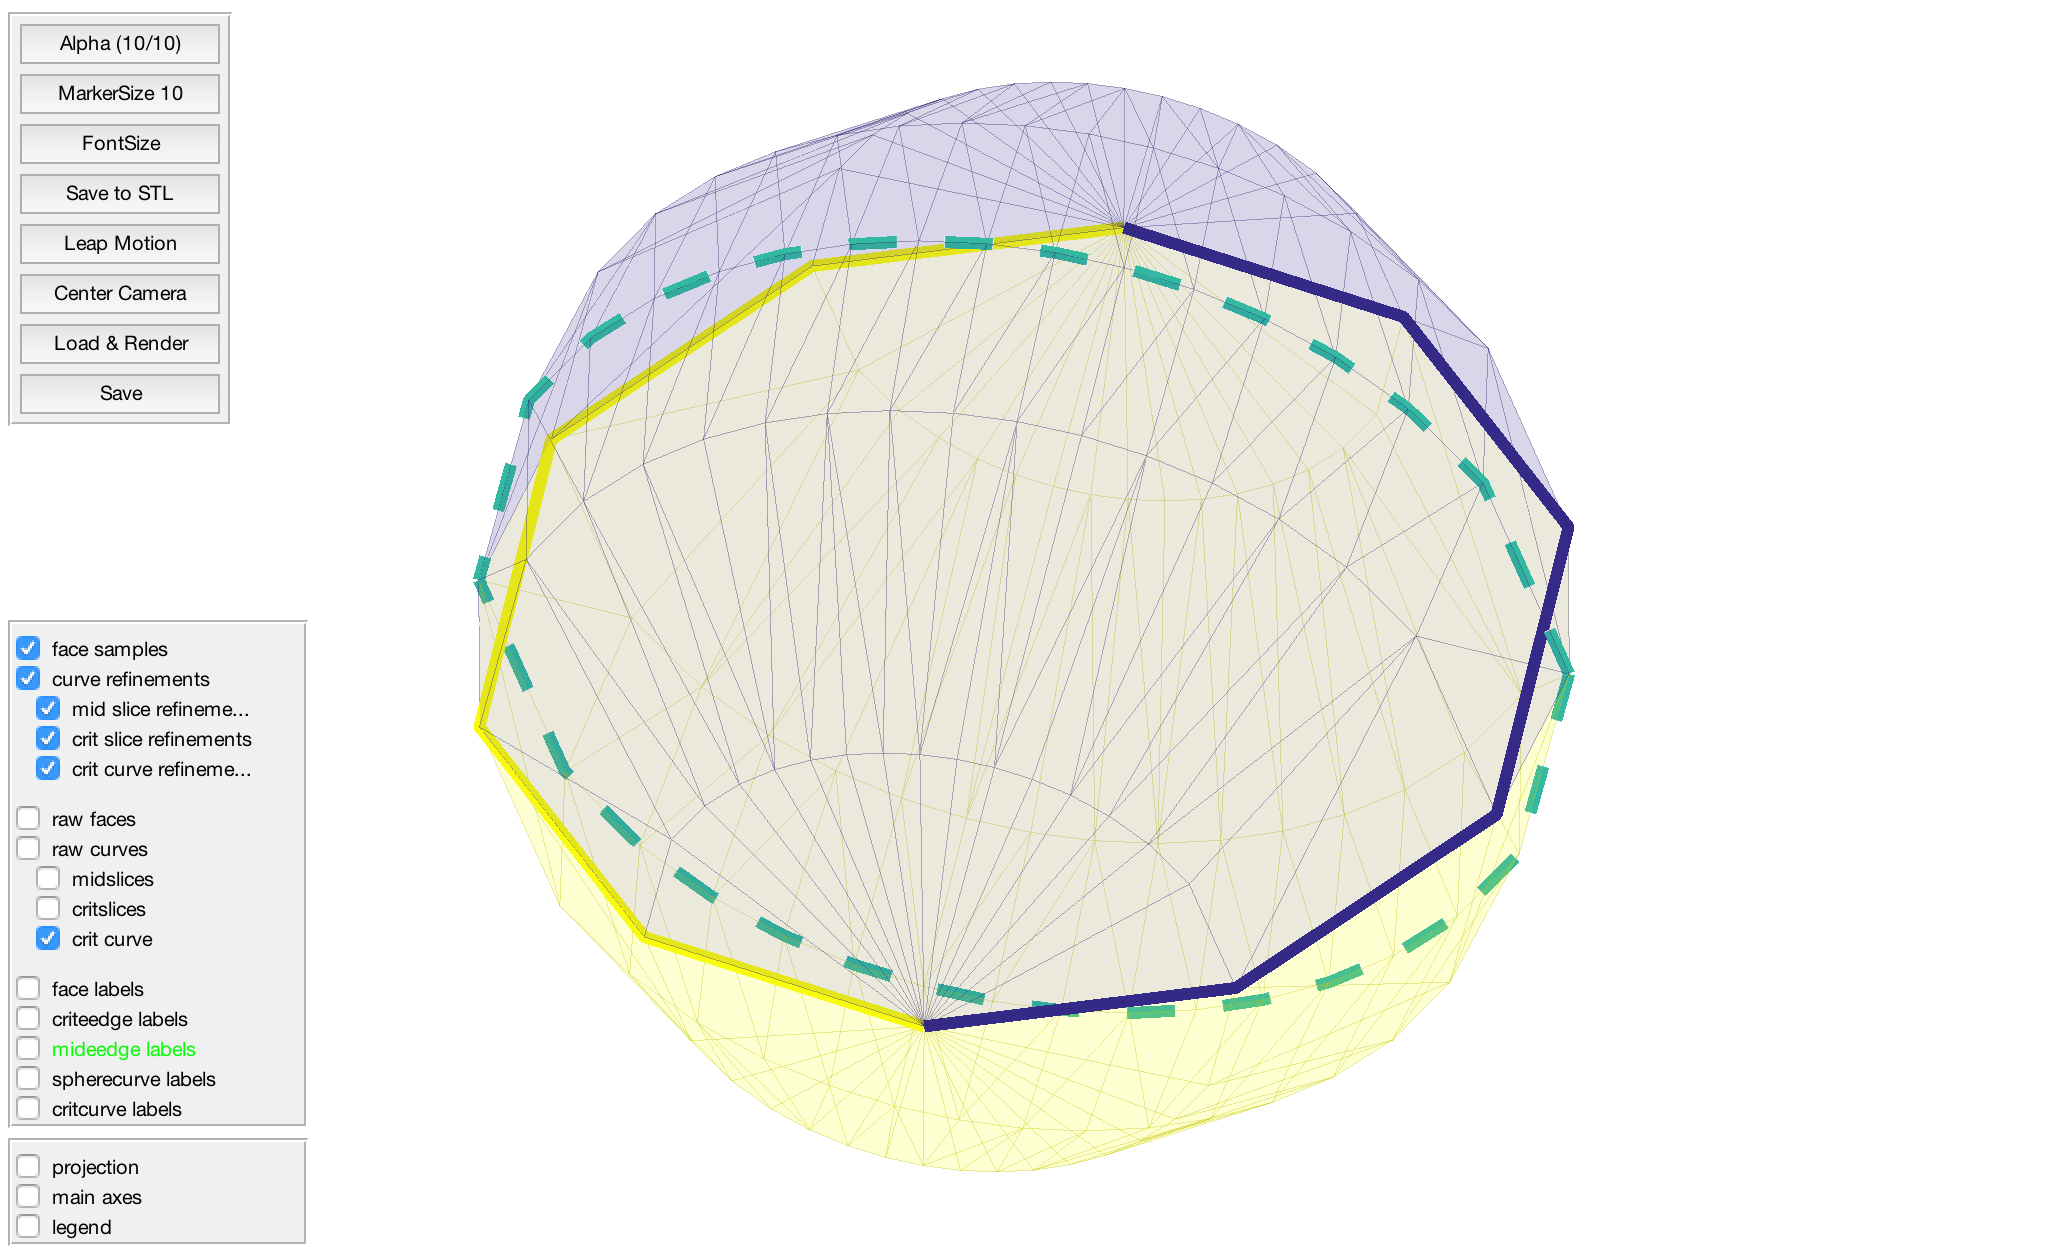
\includegraphics[width=10cm]{ad_dis_minribs.png}}
     \caption{This is an example of sampling a surface using the adaptive by distance minribs mode. To replicate this, when invoking sampler, type in {\tt sampler -m d minribs 10 -tol 0.9}}
\end{figure}

\begin{figure}[!htb]\centering
     \frame{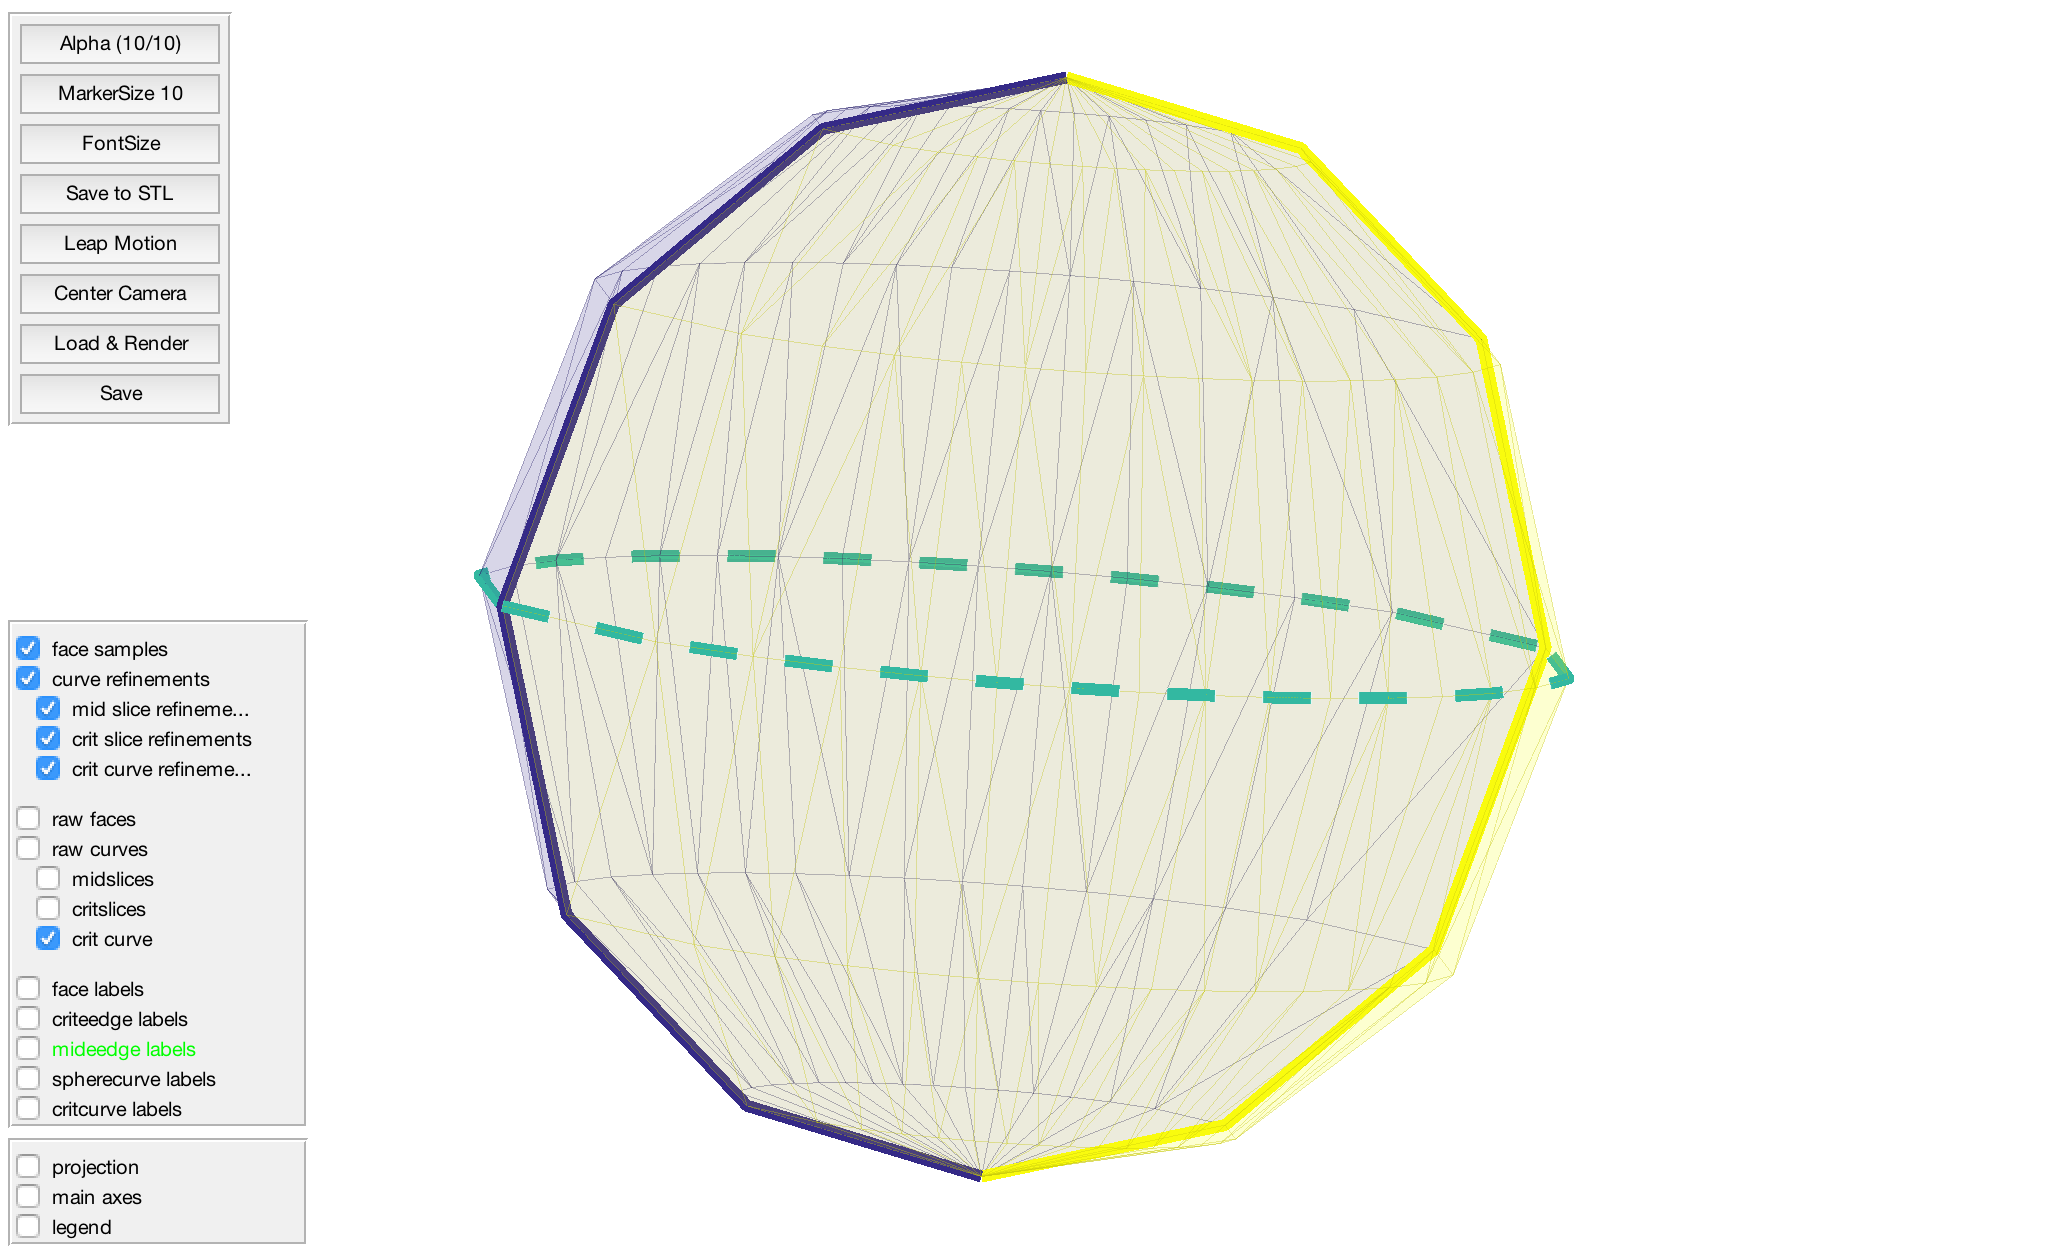
\includegraphics[width=10cm]{ad_dis_maxribs.png}}
     \caption{This is an example of sampling a surface using the adaptive by distance maxribs mode. To replicate this, when invoking sampler, type in {\tt sampler -m d maxribs 10 -tol 0.7}}
\end{figure}


\begin{figure}[!htb]\centering
     \frame{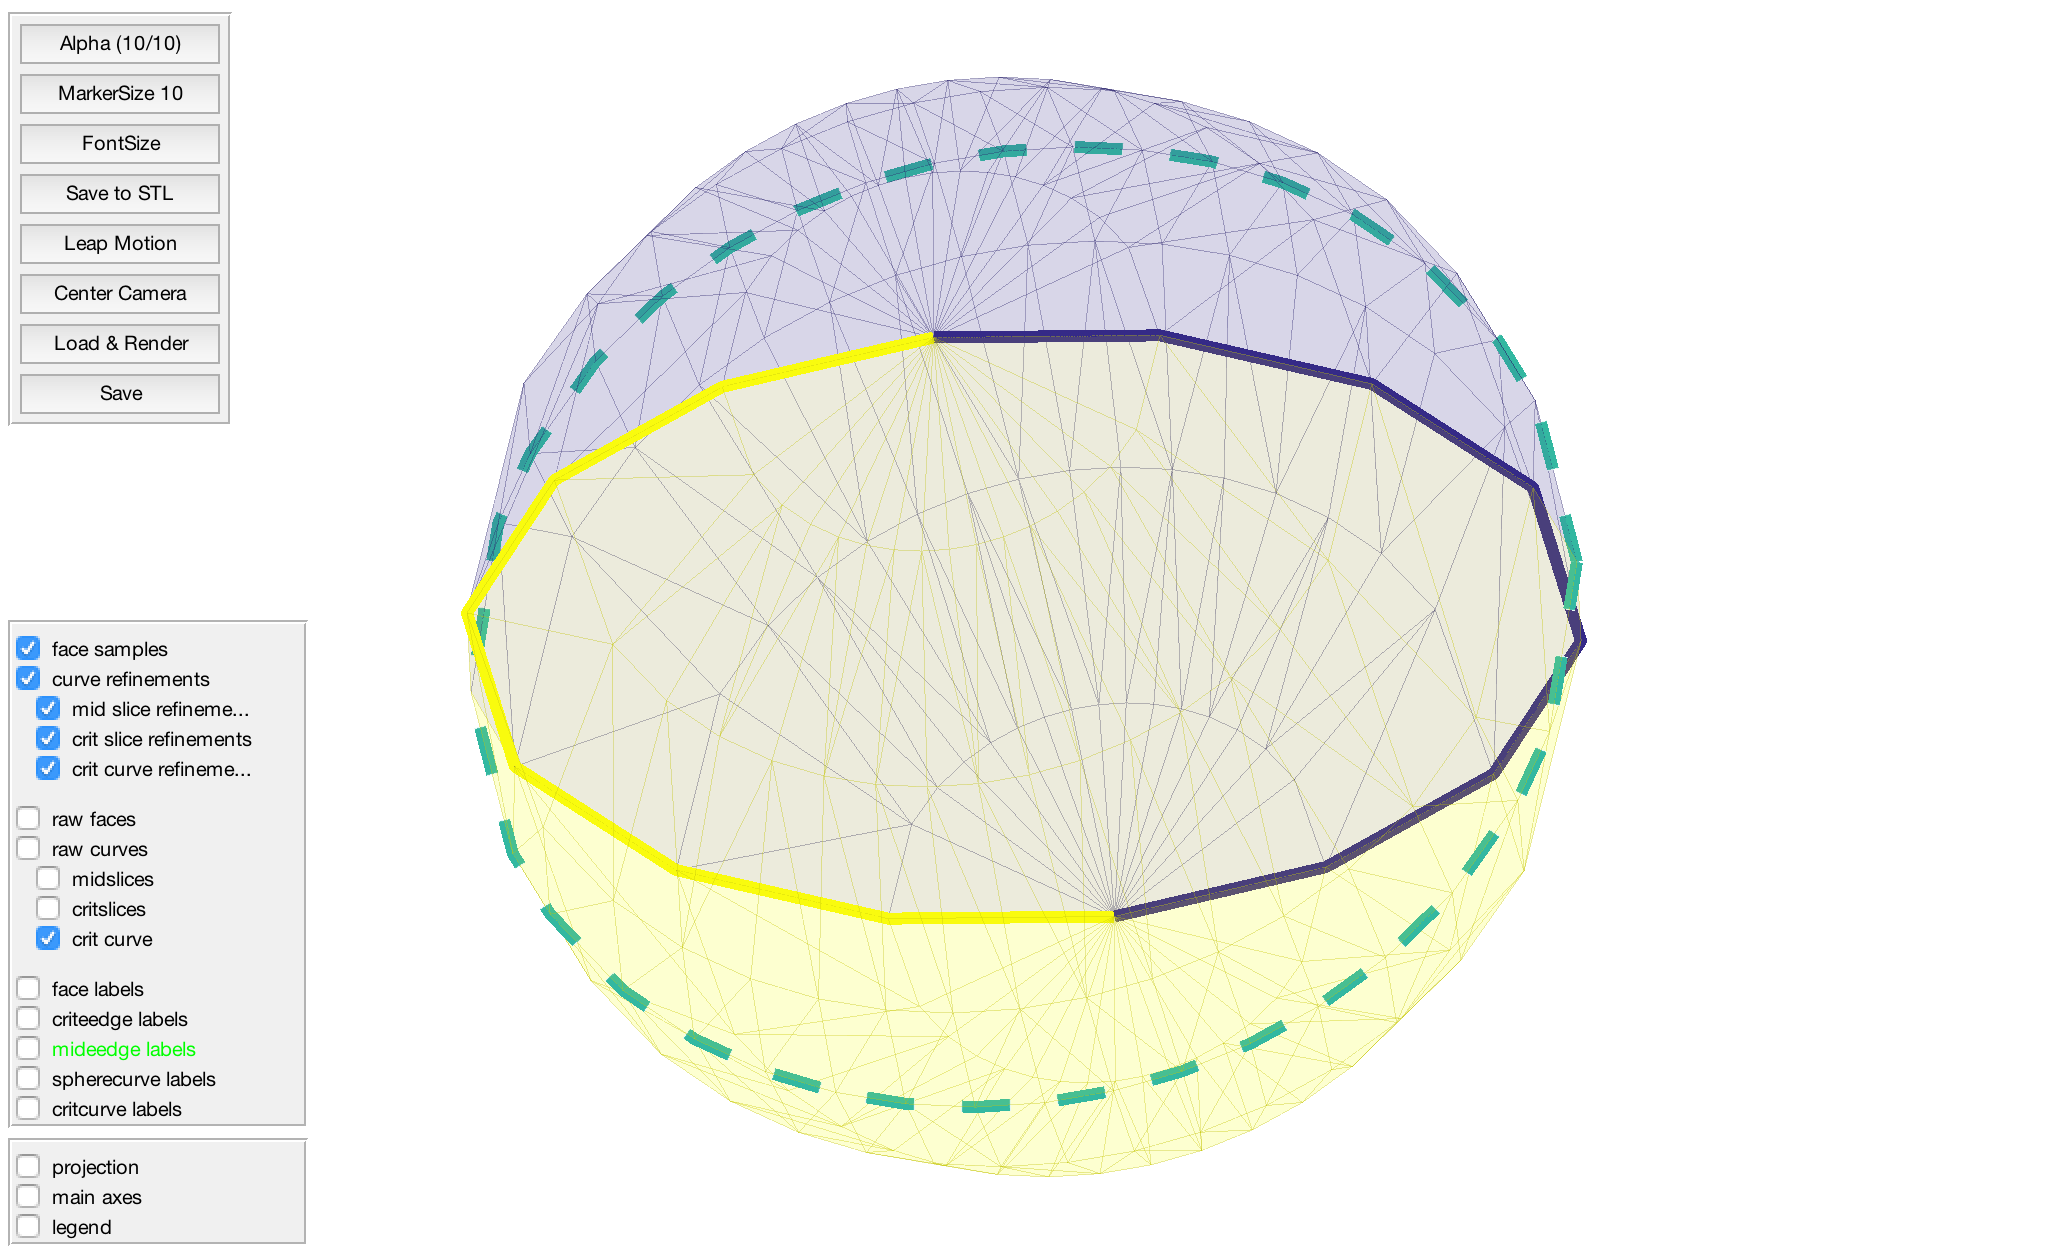
\includegraphics[width=10cm]{ad_dis_minits.png}}
     \caption{This is an example of sampling a surface using the adaptive by distance minits mode. To replicate this, when invoking sampler, type in {\tt sampler -m d minits 10 -tol 0.5}}
\end{figure}


\begin{figure}[!htb]\centering
     \frame{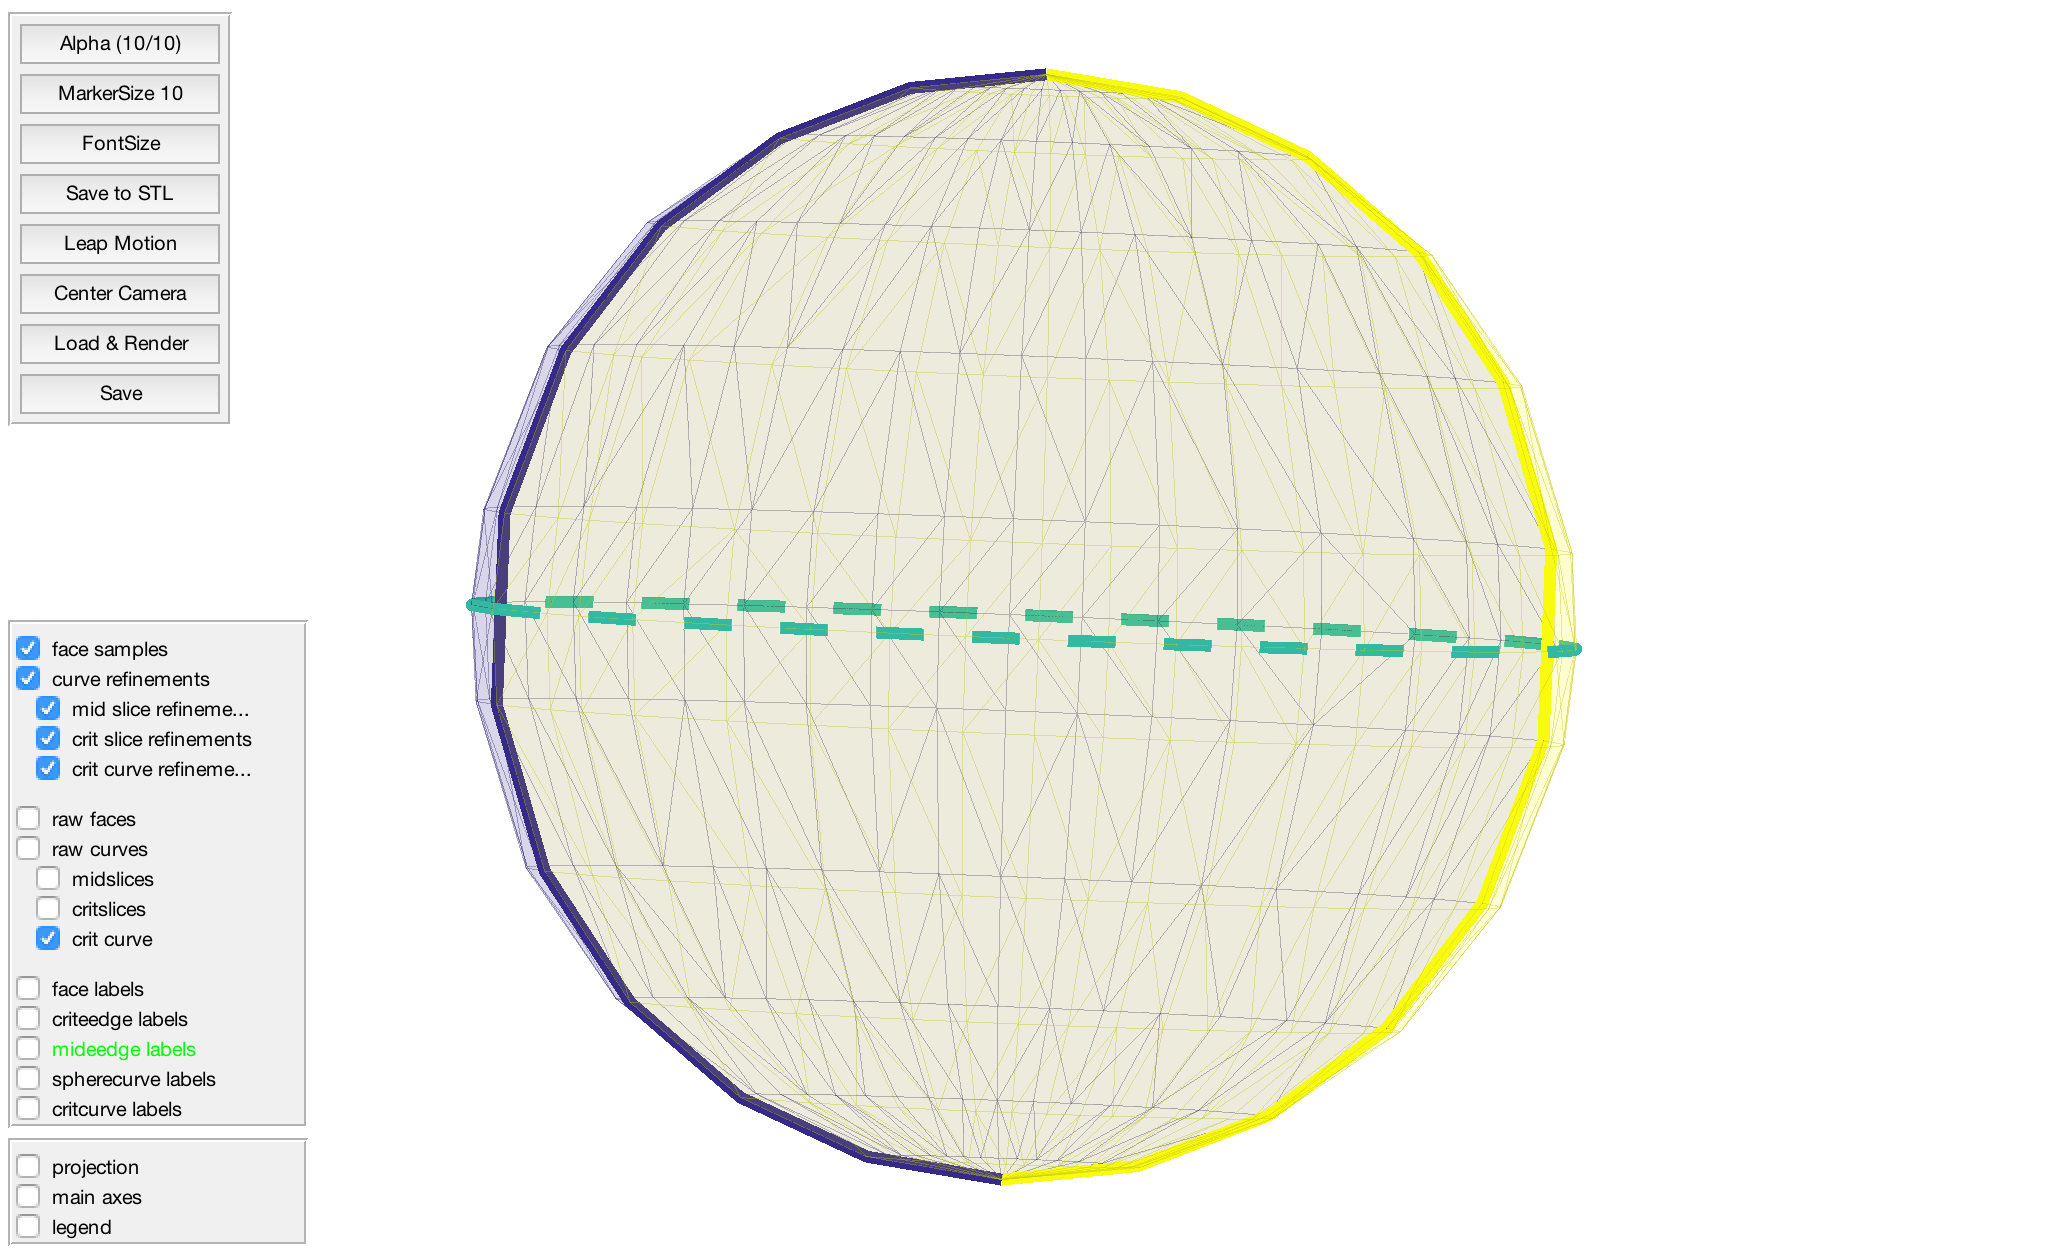
\includegraphics[width=10cm]{ad_dis_maxits.png}}
     \caption{This is an example of sampling a surface using the adaptive by distance maxits mode. To replicate this, when invoking sampler, type in {\tt sampler -m d maxits 10 -tol 0.3}}
\end{figure}





\subsubsection{Known issues with surface sampler}

The method for triangulating the faces can sometimes produce janky results.  It is known.   You'll know it too, when you see it.  If you want to help fix this, please contact Dani.  They're ready to collaborate with you!

